\documentclass{article}
\usepackage{booktabs}
\usepackage{multirow}
\usepackage{multicol}
\usepackage[table]{xcolor}
\usepackage{colortbl}
\usepackage[backend=biber,natbib=true,style=alphabetic,maxbibnames=50]{biblatex}
\addbibresource{/home/nqbh/reference/bib.bib}
\usepackage[utf8]{vietnam}
\usepackage{tocloft}
\usepackage{tcolorbox}

\setlength{\parindent}{0pt}


\usepackage{minted}

\usepackage{listings}
\usepackage{xcolor}

\lstset{
    language=C++,                    % Ngôn ngữ lập trình
    basicstyle=\ttfamily\footnotesize, % Cỡ chữ nhỏ hơn
    keywordstyle=\color{blue},        % Màu từ khóa
    commentstyle=\color{gray},        % Màu chú thích
    stringstyle=\color{red},          % Màu chuỗi ký tự
    numbers=left,                     % Hiển thị số dòng bên trái
    numberstyle=\tiny\color{gray},    % Định dạng số dòng
    stepnumber=1,                     % Mỗi dòng đều có số dòng
    breaklines=true,                   % Tự động xuống dòng nếu quá dài
    frame=single                      % Đóng khung mã nguồn
}

\renewcommand{\cftsecleader}{\cftdotfill{\cftdotsep}}
\usepackage[colorlinks=true,linkcolor=blue,urlcolor=red,citecolor=magenta]{hyperref}
\usepackage{amsmath,amssymb,amsthm,enumitem,float,graphicx,mathtools,tikz}
\usetikzlibrary{angles,calc,intersections,matrix,patterns,quotes,shadings}
\allowdisplaybreaks
\newtheorem{assumption}{Assumption}
\newtheorem{baitoan}{}
\newtheorem{cauhoi}{Câu hỏi}
\newtheorem{conjecture}{Conjecture}
\newtheorem{corollary}{Corollary}
\newtheorem{dangtoan}{Dạng toán}
\newtheorem{definition}{Definition}
\newtheorem{dinhly}{Định lý}
\newtheorem{dinhnghia}{Định nghĩa}
\newtheorem{example}{Example}
\newtheorem{ghichu}{Ghi chú}
\newtheorem{hequa}{Hệ quả}
\newtheorem{giathuyet}{Giả thuyết}
\newtheorem{chungminh}{Chứng minh}
\newtheorem{hypothesis}{Hypothesis}
\newtheorem{lemma}{Lemma}
\newtheorem{luuy}{Lưu ý}
\newtheorem{nhanxet}{Nhận xét}
\newtheorem{baitap}{Bài tập}
\newtheorem{notation}{Notation}
\newtheorem{note}{Note}
\newtheorem{principle}{Principle}
\newtheorem{problem}{Problem}
\newtheorem{proposition}{Proposition}
\newtheorem{question}{Question}
\newtheorem{remark}{Remark}
\newtheorem{theorem}{Theorem}
\newtheorem{vidu}{Ví dụ}
\usepackage[left=1cm,right=1cm,top=5mm,bottom=5mm,footskip=4mm]{geometry}
\def\labelitemii{$\circ$}
\DeclareRobustCommand{\divby}{%
	\mathrel{\vbox{\baselineskip.65ex\lineskiplimit0pt\hbox{.}\hbox{.}\hbox{.}}}%
}
\setlist[itemize]{leftmargin=*}
\setlist[enumerate]{leftmargin=*}

\title{CHUYÊN ĐỀ: LÝ THUYẾT ĐỒ THỊ} 
\author{Đặng Phúc An Khang\footnote{ E-mail: {\tt ankhangluonvuituoi@gmail.com}. Tây Ninh, Việt Nam.}}
\date{\today}

\begin{document}
\maketitle
\begin{abstract}
	
	
	\textbf{Code:}
	\begin{quote}
		\begin{itemize}
			\item C{\tt/}C++: \url{https://github.com/GrootTheDeveloper/OLP-ICPC/tree/master/2025/C%2B%2B}.
			\item Python: \url{}\\
		\end{itemize}
	\end{quote}
	
	\textbf{Tài khoản trên các Online Judge:}
	\begin{quote}
    	\begin{itemize}
			\item Codeforces: \url{https://codeforces.com/profile/vuivethoima}.
			\item VNOI: \url{oj.vnoi.info/user/Groot}.
			\item IUHCoder: \url{oj.iuhcoder.com/user/ankhang2111}.
			\item MarisaOJ: \url{https://marisaoj.com/user/grootsiuvip/submissions}.
			\item CSES: \url{https://cses.fi/user/212174}.
			\item UMTOJ: \url{sot.umtoj.edu.vn/user/grootsiuvip}.
			\item SPOJ: \url{www.spoj.com/users/grootsiuvip/}.
			\item POJ: \url{http://poj.org/userstatus?user_id=vuivethoima}.
			\item ATCoder: \url{https://atcoder.jp/users/grootsiuvip}
			\item OnlineJudge.org: \url{vuivethoima}
			\item updating...
		\end{itemize}
	\end{quote}
    
\end{abstract}
\tableofcontents

%------------------------------------------------------------------------------%

\section{Preliminaries -- Kiến thức chuẩn bị}

\textbf{\textsf{Resources -- Tài nguyên.}}
\begin{enumerate}
	\item \cite{CP10}. \textit{CP10. Competitive Programming} \url{https://drive.google.com/drive/folders/1MTEVHT-7nBnMJ7C9LgyAR_pEVSE3FlKz?fbclid=IwAR3TovIj2rKCRe1a4oZxW-LQCoEoVkipVAvCzwrr0nJ6GzcAd47P6LO1Rwc}
	
	\item \cite{cp-algorithms}. \textit{Algorithms for Competitive Programming} \url{https://cp-algorithms.com}

    \item \cite{VNOI-WIKI}. \textit{Thư viện VNOI} \url{https://wiki.vnoi.info}



\end{enumerate}


%------------------------------------------------------------------------------%
\section{Kiến thức}
\subsection{Giới thiệu về đồ thị và thuật toán DFS}

\subsubsection{Lý thuyết đồ thị là gì?}

\begin{dinhnghia}
    Lý thuyết đồ thị là một nhánh của toán học, cụ thể thuộc toán rời rạc. Lý thuyết đồ thị chuyên nghiên cứu các bài toán liên quan đến việc biểu diễn và phân tích các sự vật, hiện tượng hoặc trạng thái có mối quan hệ lẫn nhau thông qua mô hình đồ thị.
\end{dinhnghia}
\begin{vidu}
    Mạng lưới giao thông, cây phả hệ (cây gia phả), mạng máy tính, sơ đồ tổ chức, v.v.
\end{vidu}

\subsubsection{Một số khái niệm căn bản trong lý thuyết đồ thị}

\begin{enumerate}
    \item \textbf{Đỉnh:} Được biểu diễn nhằm mục đích thể hiện sự vật, sự việc hay một trạng thái.
    \item \textbf{Cạnh:} Biểu diễn cho mối quan hệ giữa 2 đỉnh với nhau. \textbf{Lưu ý:} Giữa 2 đỉnh trong đồ thị có thể có cạnh, không có, hoặc có thể có nhiều cạnh với nhau. Cạnh được chia thành 2 dạng:
    \begin{enumerate}
        \item \textbf{Cạnh vô hướng:} Nếu một cạnh vô hướng nối 2 đỉnh $u$ và $v$, thì $u$ có thể đến $v$ trực tiếp vầ ngược lại.
        \item \textbf{Cạnh có hướng:} Nếu một cạnh có hướng nối từ đỉnh $u$ đến đỉnh $v$, thì ta có thể đi trực tiếp từ $u$ đến $v$, nhưng không thể đi ngược lại từ $v$ đến $u$ trừ khi có một cạnh khác từ $v$ đến $u$.
    \end{enumerate}
    \item \textbf{Đường đi:} Một đường đi là một danh sách các đỉnh $x_1, x_2, x_3, x_4,\dots, x_k$. Trong đó 2 đỉnh $x_i$ và $x_{i + 1}$ thì có một đường nối trực tiếp để đi từ $x_i$ $\rightarrow$ $x_{i + 1}$.
    \item \textbf{Trọng số:} Là một giá trị trên cạnh (hoặc trên đỉnh) nhằm thể hiện một thông số nào đó với bài toán ta đang xét.
\end{enumerate}

\subsubsection{Danh sách kề}

Một trong những cách phổ biến để biểu diễn đồ thị là sử dụng \textbf{danh sách kề (adjacency list)}. Cách biểu diễn này đặc biệt hiệu quả đối với đồ thị thưa \href{https://en.m.wikipedia.org/wiki/Sparse_graph}{(sparse graph)}.


Cụ thể, ta sử dụng cấu trúc dữ liệu \texttt{vector<int> adj[u]} trong C++, trong đó:

\begin{itemize}
    \item Mỗi phần tử \texttt{adj[u]} là một vector chứa các đỉnh kề với đỉnh $u$.
    \item Nghĩa là nếu có cạnh nối từ đỉnh $u$ đến đỉnh $v$ thì $v$ sẽ xuất hiện trong \texttt{adj[u]}.
    \item Đối với đồ thị vô hướng, nếu có cạnh giữa $u$ và $v$ thì cả $v \in \texttt{adj}[u]$ và $u \in \texttt{adj}[v]$.
\end{itemize}

\textbf{Ví dụ:}

Giả sử đồ thị vô hướng có các cạnh: $(1,2)$, $(1,3)$, $(2,4)$ thì danh sách kề sẽ là:

\begin{align*}
\texttt{adj[1]} &= \{2, 3\} \\
\texttt{adj[2]} &= \{1, 4\} \\
\texttt{adj[3]} &= \{1\} \\
\texttt{adj[4]} &= \{2\}
\end{align*}

\begin{figure}[H]
    \centering
    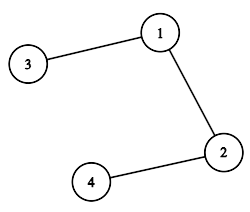
\includegraphics[width=0.2\textwidth]{img/b1/adjlist.png}
    \caption{Minh họa danh sách kề của đồ thị vô hướng vừa mô tả}
    \label{fig:adjlist}
\end{figure}

Cách biểu diễn này có độ phức tạp về bộ nhớ là $\mathcal{O}(n + m)$, với $n$ là số đỉnh và $m$ là số cạnh.

\subsubsection{Chu trình (Cycle)}
\begin{dinhnghia}
    Một \textbf{chu trình} là một đường đi bắt đầu và kết thúc tại cùng một đỉnh, trong đó không có đỉnh nào khác (ngoại trừ đỉnh đầu/cuối) được lặp lại.
\end{dinhnghia}
    \begin{itemize}
        \item Trong đồ thị vô hướng: chu trình là dãy đỉnh $v_1 \rightarrow v_2 \rightarrow \dots \rightarrow v_k \rightarrow v_1$ với $k \geq 3$.
        \item Trong đồ thị có hướng: các cung phải có hướng phù hợp với trình tự chu trình.
    \end{itemize}
    
    Một chu trình được gọi là \textit{chu trình đơn giản} nếu không có cạnh hoặc đỉnh nào bị lặp lại (trừ đỉnh đầu/cuối).
    
\begin{figure}[H]
    \centering
    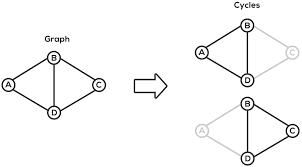
\includegraphics[width=0.4\textwidth]{img/b1/cycle.png}
    \caption{Minh họa chu trình của đồ thị vô hướng}
    \label{fig:cycle}
\end{figure}

\subsubsection{Thành phần liên thông \href{https://www.geeksforgeeks.org/dsa/strongly-connected-components/}{(Connected Component)}}
\begin{dinhnghia}

    Một \textbf{thành phần liên thông} là một tập con các đỉnh sao cho giữa mọi cặp đỉnh trong đó đều tồn tại một đường đi.
\end{dinhnghia}
    
\begin{itemize}
    \item Với đồ thị vô hướng: liên thông nếu có đường đi giữa mọi cặp đỉnh.
    \item Với đồ thị có hướng:
        \begin{itemize}
            \item \textit{Liên thông mạnh} nếu tồn tại đường đi theo chiều từ mọi đỉnh đến mọi đỉnh khác.
            \item \textit{Liên thông yếu} nếu bỏ hướng trên các cạnh thì đồ thị trở nên liên thông.
        \end{itemize}
\end{itemize}

\begin{figure}[H]
    \centering
    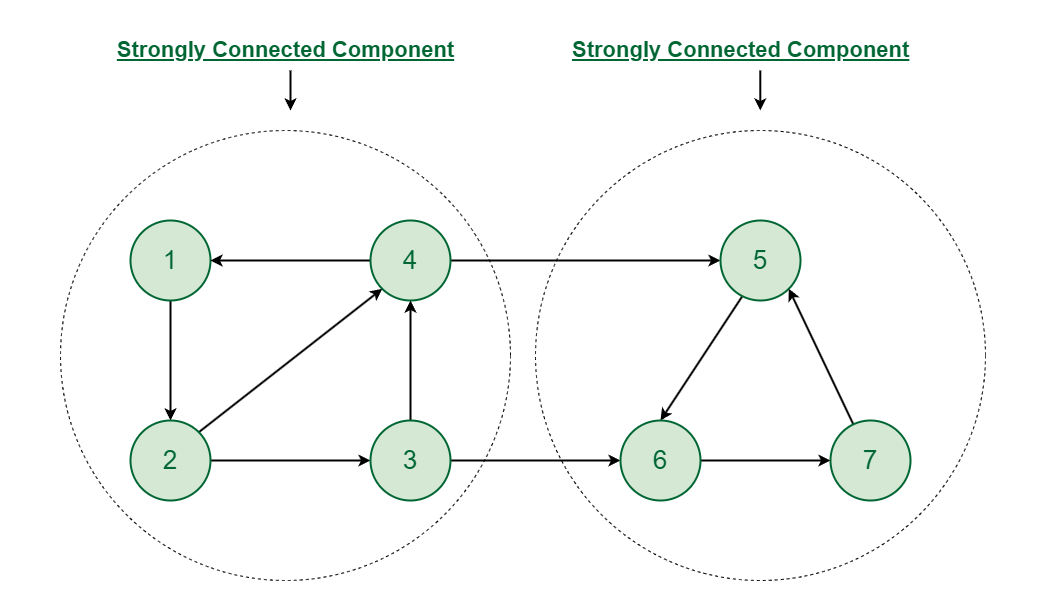
\includegraphics[width=0.4\textwidth]{img/b1/SCC.png}
    \caption{Minh họa thành phần liên thông mạnh của đồ thị có hướng}
    \label{SCC}
\end{figure}

\subsubsection{Bậc của đỉnh (Degree)}
\begin{itemize}
    \item Trong đồ thị vô hướng, bậc của một đỉnh là số cạnh nối với nó.
    \item Trong đồ thị có hướng:
        \begin{itemize}
            \item \textit{Bậc vào} (in-degree): số cung đi vào đỉnh.
            \item \textit{Bậc ra} (out-degree): số cung đi ra từ đỉnh.
        \end{itemize}
\end{itemize}

\subsubsection{Đường đi đơn giản (Simple Path)}
Một \textbf{đường đi đơn giản} là đường đi không đi qua một đỉnh nào hai lần (trừ khi là chu trình).

\subsubsection{Cây (Tree)}
\begin{dinhnghia}
    
    Một \textbf{cây} là một đồ thị vô hướng liên thông và không có chu trình.
    
\end{dinhnghia}
Tính chất quan trọng của cây:
\begin{itemize}
    \item Với $n$ đỉnh, cây có đúng $n - 1$ cạnh.
    \item Có duy nhất một đường đi giữa hai đỉnh bất kỳ.
\end{itemize}

\begin{figure}[H]
    \centering
    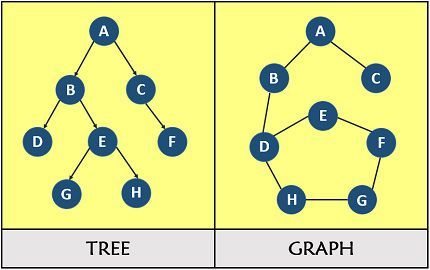
\includegraphics[width=0.4\textwidth]{img/b1/treegraph.png}
    \caption{Phân biệt Cây và Đồ thị (không phải cây)}
    \label{treegraph}
\end{figure}

\subsubsection{Đồ thị vô chu trình (Acyclic Graph).}
Đồ thị gọi là \textbf{vô chu trình} nếu không tồn tại chu trình nào trong nó.
\begin{itemize}
    \item Với đồ thị \textbf{vô hướng}, một đồ thị được xem là \textbf{Acyclic Graph} nếu không tồn tại dãy các đỉnh $v_1 \rightarrow v_2 \rightarrow \dots \rightarrow v_k \rightarrow v_1$ với $k \geq 3$ và các cạnh liên tiếp nối các đỉnh đó.
    \item Một đồ thị vô hướng đơn giản gồm hai đỉnh được nối với nhau bằng một cạnh cũng là một \textbf{Acyclic Graph}, vì không tồn tại chu trình nào (phải có ít nhất 3 đỉnh để hình thành chu trình trong đồ thị vô hướng).
    \item Đồ thị có hướng vô chu trình gọi là \textbf{DAG} (Directed Acyclic Graph). Nghĩa là một đồ thị có hướng không chứa bất kỳ chu trình nào tuân theo chiều các cung.
    \item Cây là một DAG, nhưng không phải tất cả DAG đều là cây.
\end{itemize}

\begin{figure}[H]
    \centering
    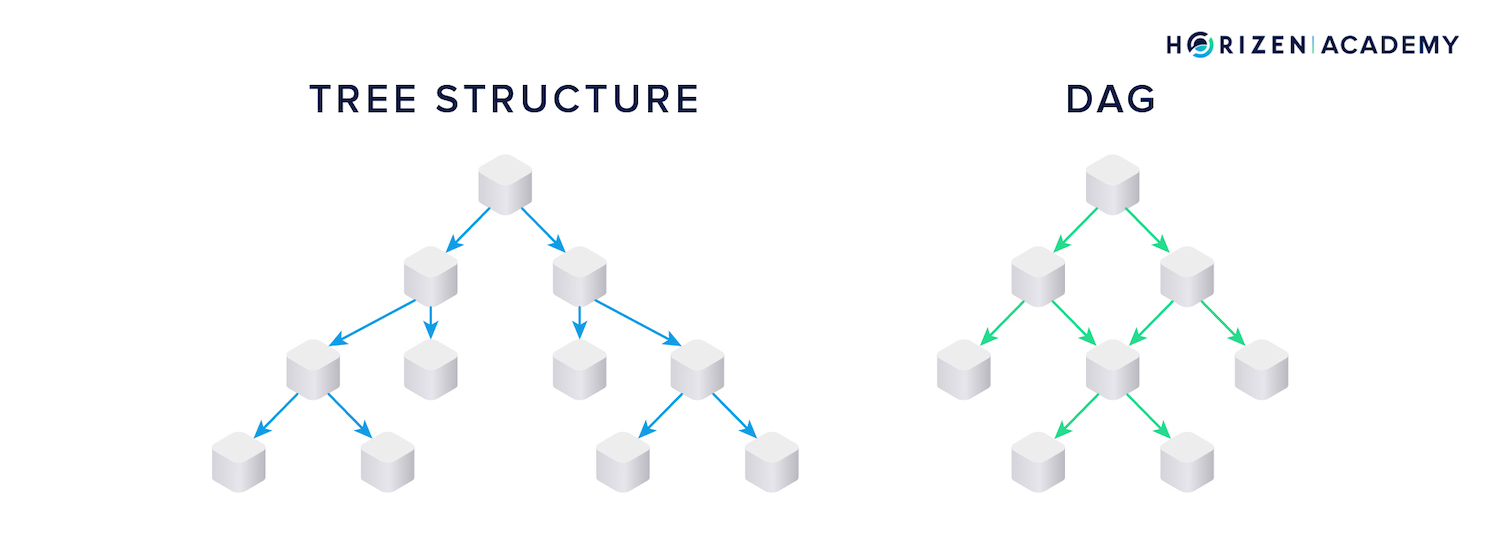
\includegraphics[width=0.6\textwidth]{img/b1/treevsdag.jpg}
    \caption{Phân biệt Cây và DAG}
\end{figure}

\subsubsection{Đồ thị đơn (Simple Graph).}
Đồ thị đơn là đồ thị không có \emph{cạnh lặp} giữa cùng một cặp đỉnh và không có \emph{khuyên} (loop – cạnh nối đỉnh với chính nó).

\subsubsection{Đa đồ thị (Multigraph).}
Đa đồ thị cho phép tồn tại \emph{nhiều cạnh song song} giữa hai đỉnh và/hoặc khuyên.  
Thường dùng để mô hình hoá các mạng có nhiều kênh kết nối.

\begin{figure}[H]
    \centering
    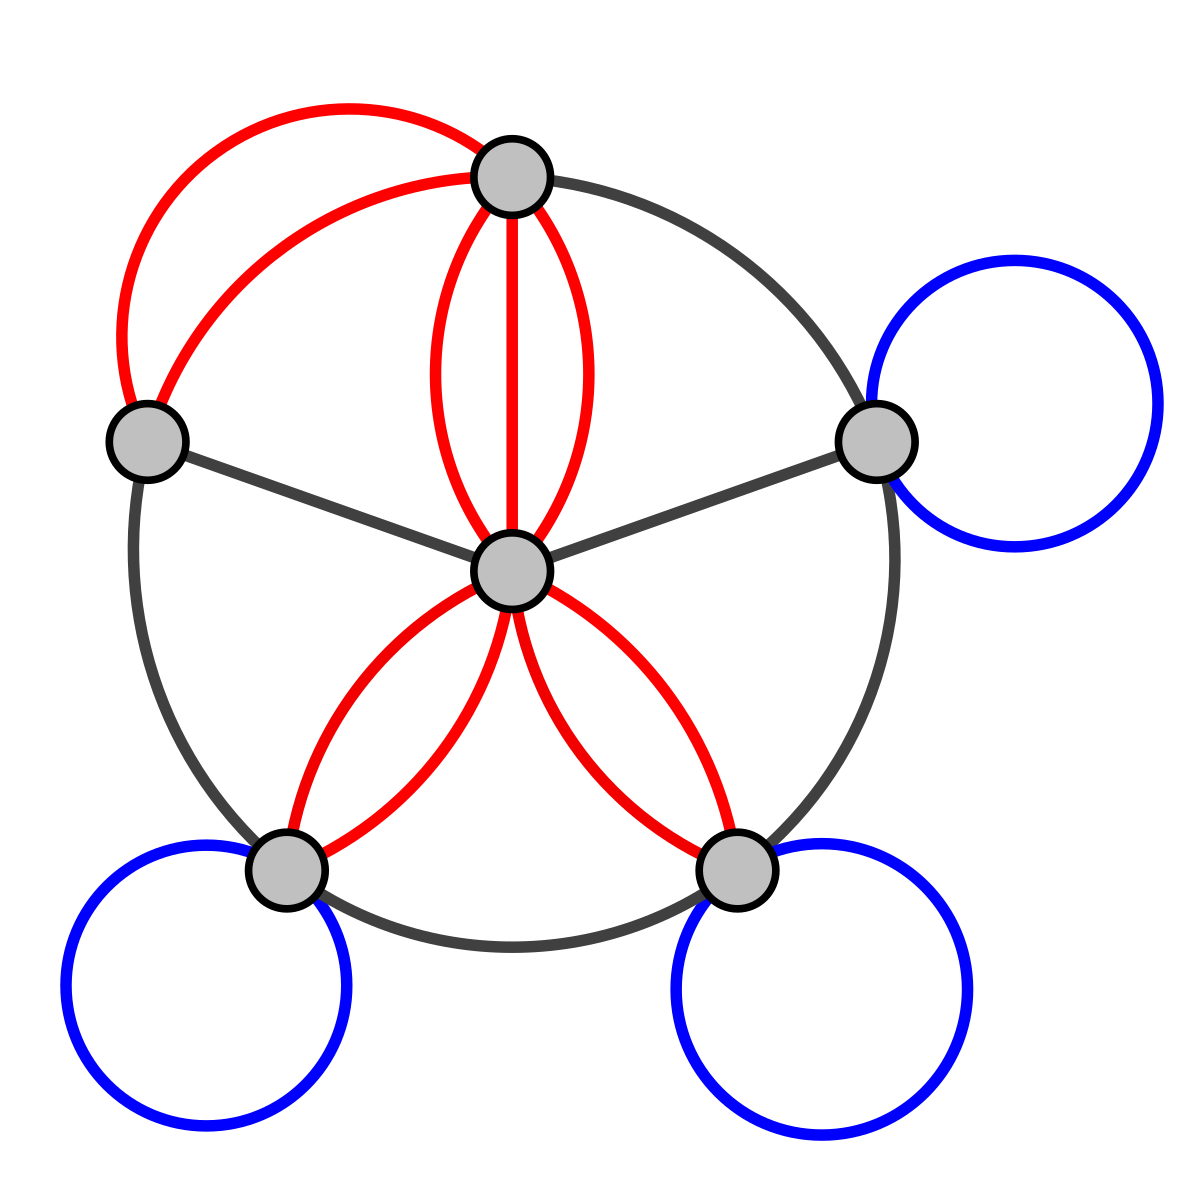
\includegraphics[width=0.2\textwidth]{img/b1/multigraph.png}
    \caption{Minh họa Đa đồ thị}
    \label{multigraph}
\end{figure}

\subsubsection{Đồ thị đầy đủ (Complete Graph).}
Đồ thị vô hướng \(K_n\) có \(n\) đỉnh, trong đó mọi cặp đỉnh phân biệt đều được nối bởi một cạnh. 

Số cạnh là \(\dfrac{n(n-1)}{2}\).  

Đồ thị có hướng đầy đủ có \(n(n-1)\) cung.

\begin{figure}[H]
    \centering
    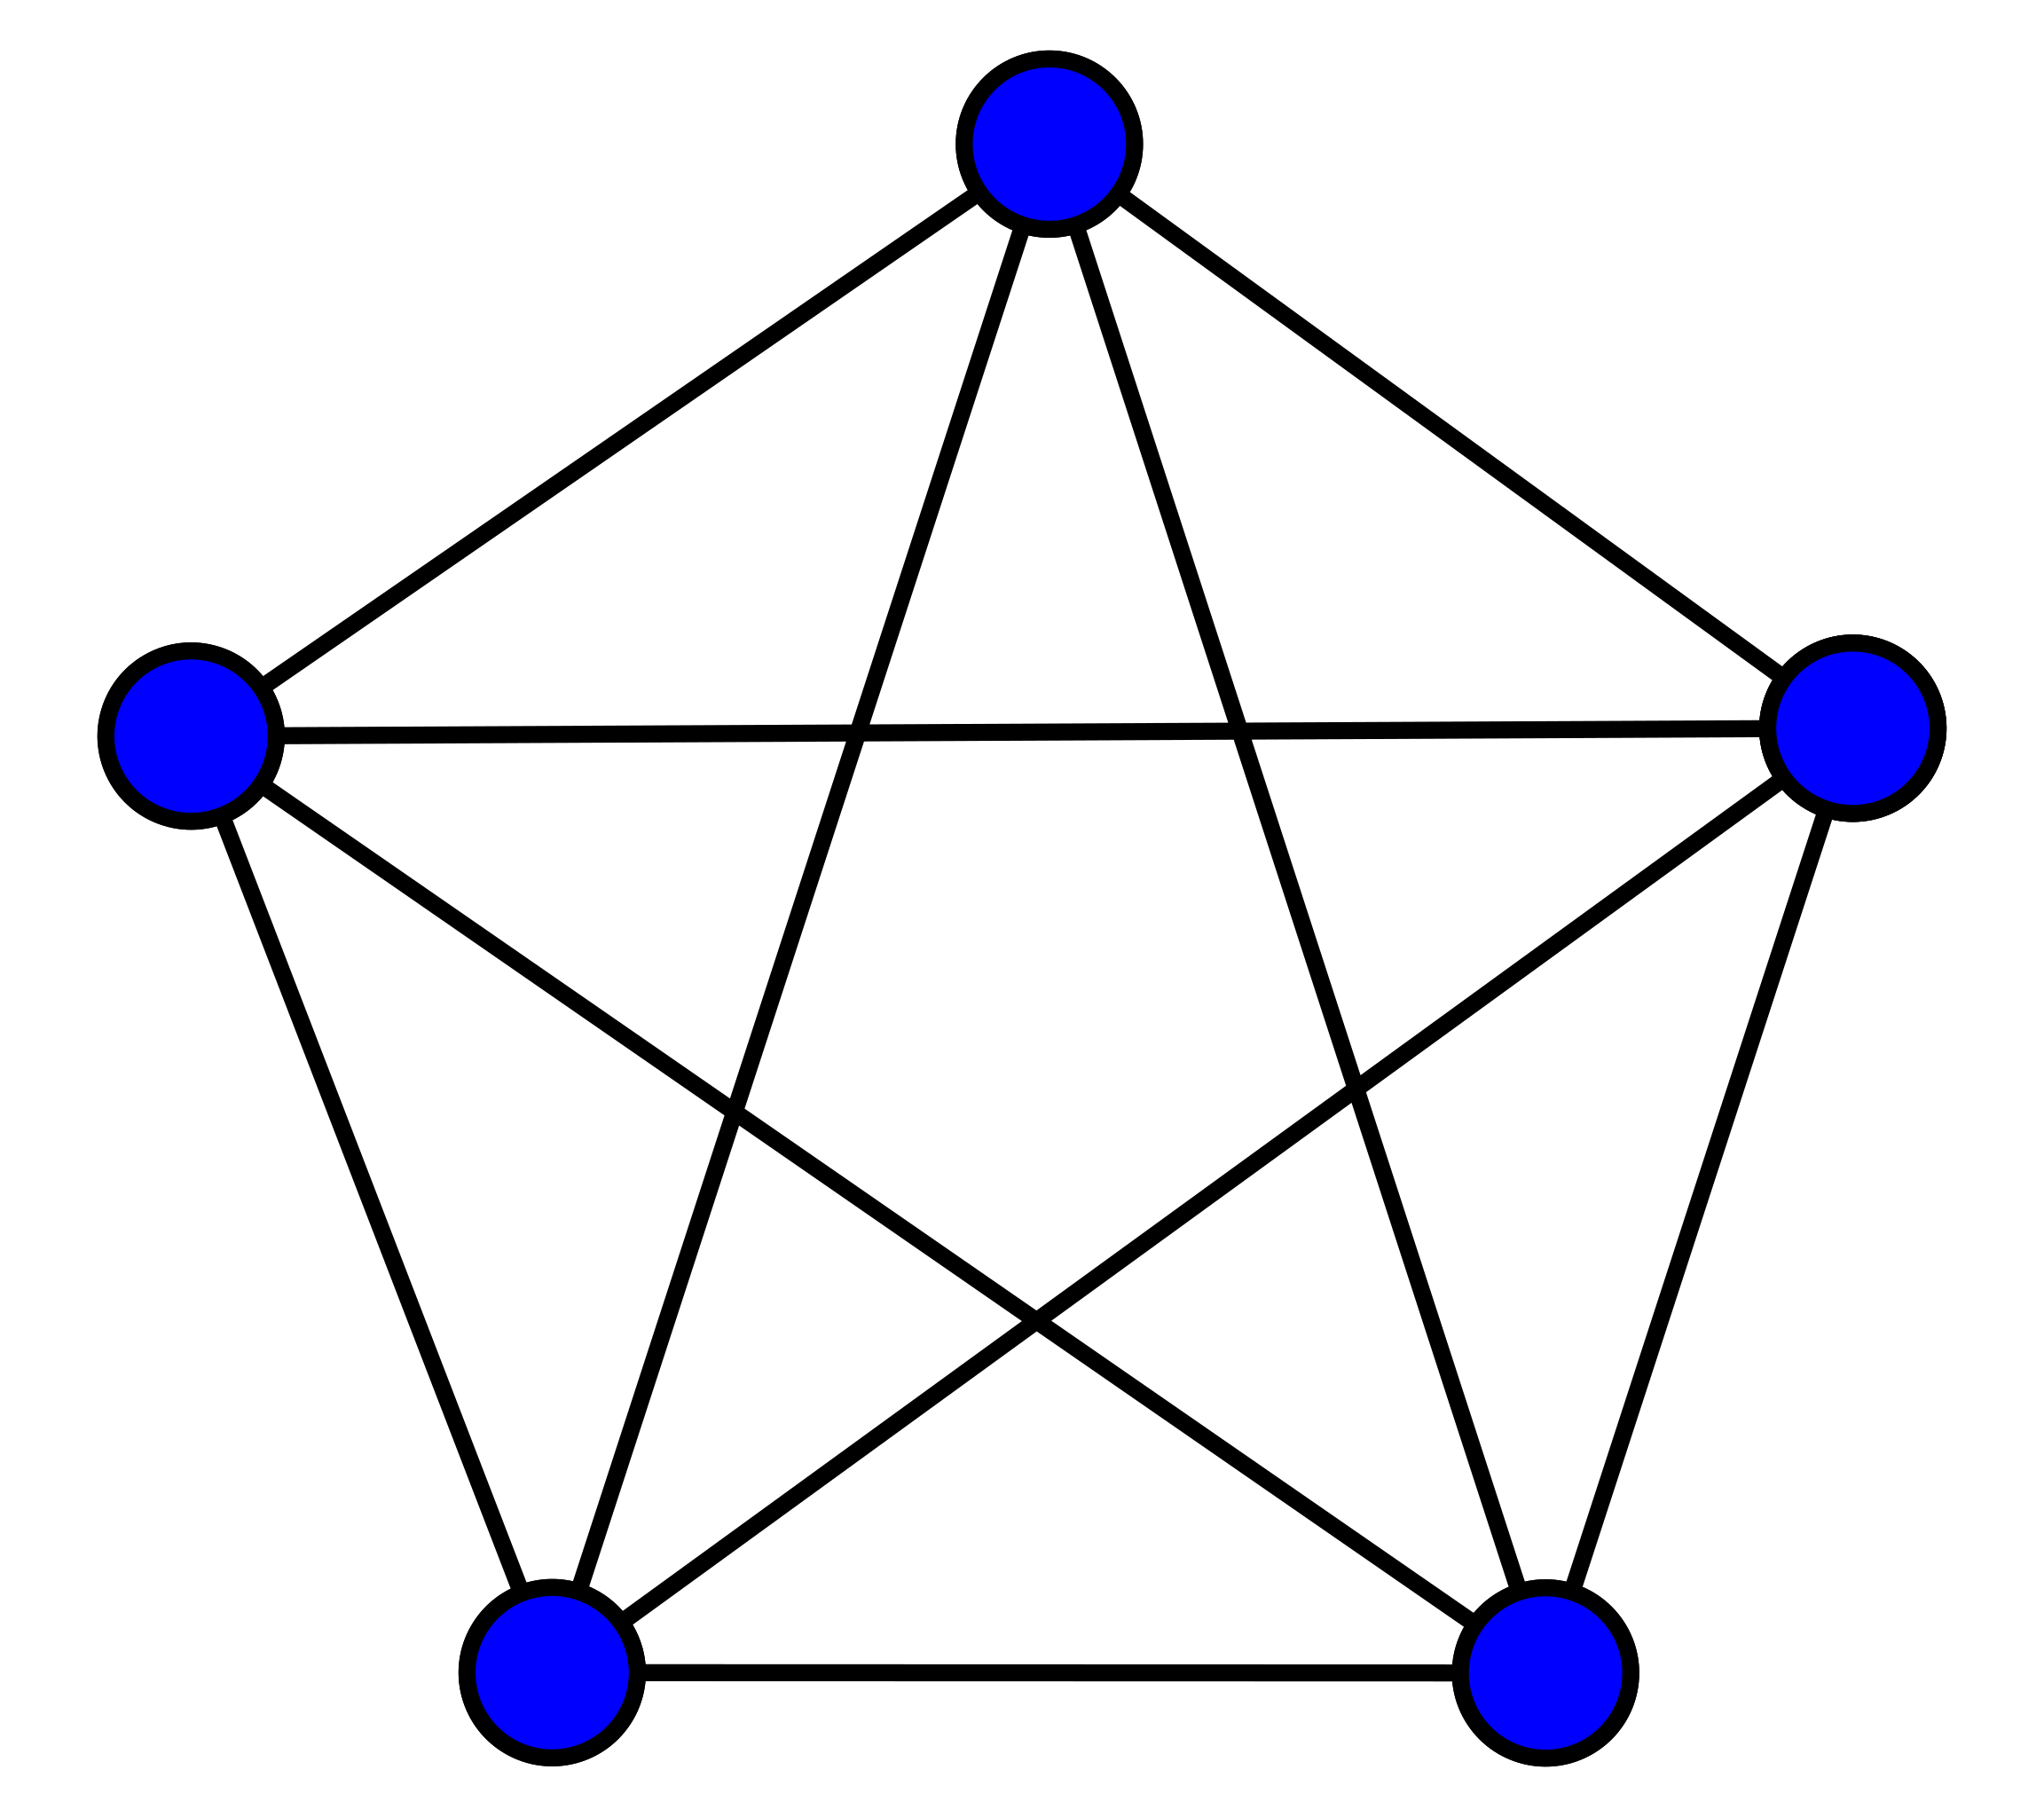
\includegraphics[width=0.2\textwidth]{img/b1/CG.png}
    \caption{Minh họa đồ thị đầy đủ}
    \label{CG}
\end{figure}

\subsubsection{Đồ thị hai phía (Bipartite Graph).}
Một \textbf{đồ thị hai phía} là đồ thị mà tập đỉnh có thể chia thành hai tập rời $U$ và $V$ sao cho mọi cạnh đều nối một đỉnh từ $U$ đến một đỉnh từ $V$.

\begin{figure}[H]
    \centering
    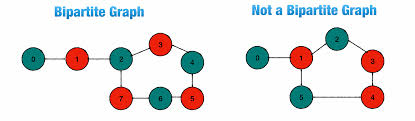
\includegraphics[width=0.5\textwidth]{img/b1/biparitegraph.png}
    \caption{Phân biệt đồ thị hai phía}
    \label{biparite}
\end{figure}

\subsubsection{Đồ thị hai phía đầy đủ (Complete Bipartite Graph).}
Cho hai tập đỉnh rời \(U\) và \(V\) với \(|U| = m,\;|V| = n\).  
Đồ thị \(K_{m,n}\) chứa mọi cạnh nối một đỉnh của \(U\) với một đỉnh của \(V\) và \emph{không có cạnh nội bộ} trong \(U\) hay \(V\).  
Tổng số cạnh: \(m\,n\).

\begin{figure}[H]
    \centering
    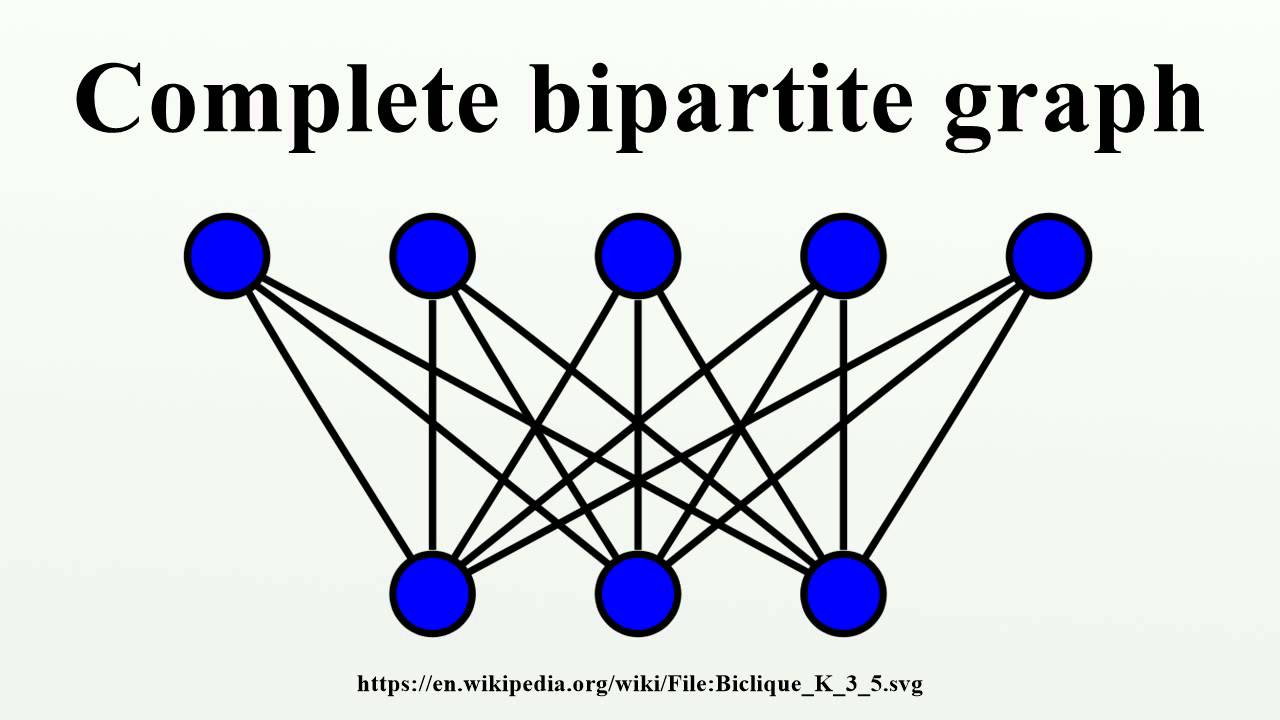
\includegraphics[width=0.4\textwidth]{img/b1/completebiparitegraph.png}
    \caption{Minh họa đồ thị hai phía đầy đủ}
    \label{CBG}
\end{figure}

\subsubsection{Đồ thị vòng (Cycle Graph)}
Đồ thị vòng ký hiệu \(C_n\;(n \ge 3)\) là đồ thị vô hướng gồm \(n\) đỉnh
\(\{v_1,v_2,\dots ,v_n\}\) và \(n\) cạnh
\[
E = \bigl\{\{v_1,v_2\},\{v_2,v_3\},\dots ,\{v_{n-1},v_n\},\{v_n,v_1\}\bigr\}.
\]

\begin{itemize}
    \item Mỗi đỉnh có bậc \(2\) – \(C_n\) là đồ thị \(2\)-chính quy.
    \item \(C_n\) chứa đúng một chu trình đơn giản độ dài \(n\).
    \item \(C_n\) là \textbf{bipartite} khi và chỉ khi \(n\) chẵn.
    \item Số cạnh \(m = n\); số đỉnh \(n\); đường kính (diameter)  
          \(\operatorname{diam}(C_n) = \bigl\lfloor n/2 \bigr\rfloor\).
    \item Tồn tại cây khung nhỏ nhất với trọng số tổng bằng \(n-1\) nếu mọi cạnh có trọng số \(1\).
\end{itemize}

\begin{figure}[H]
    \centering
    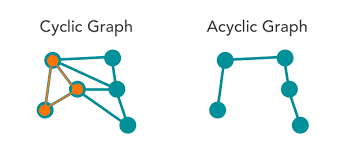
\includegraphics[width=0.4\textwidth]{img/b1/CGvsAG.png}
    \caption{Minh họa CG và AG}

\end{figure}
\subsubsection{Rừng (Forest).}
Một \textbf{rừng} là đồ thị vô hướng \emph{không chứa chu trình} nhưng \emph{không nhất thiết liên thông}.  
Mỗi thành phần liên thông của rừng là một \textbf{cây}.  
Nếu rừng có \(c\) cây và \(n\) đỉnh, nó có đúng \(n-c\) cạnh.


\begin{figure}[H]
    \centering
    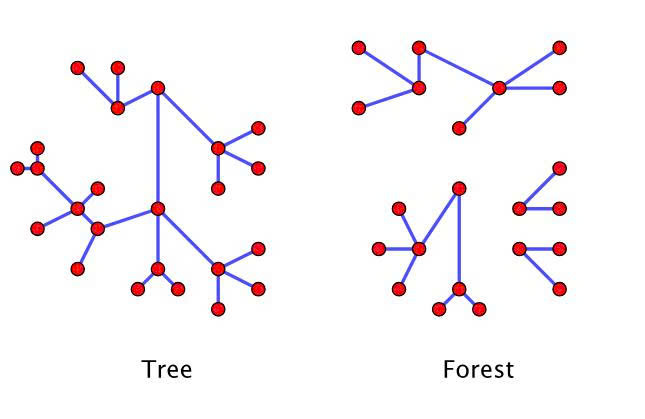
\includegraphics[width=0.4\textwidth]{img/b1/treevsforest.jpg}
    \caption{Tree vs Forest}    
\end{figure}


\subsection{Thuật toán DFS}

Thuật toán DFS (Depth-First Search – Duyệt theo chiều sâu) là một trong những thuật toán cơ bản để duyệt hoặc tìm kiếm trên đồ thị. Ý tưởng chính là xuất phát từ một đỉnh ban đầu, đi sâu theo từng nhánh con của đồ thị cho đến khi không còn đỉnh nào có thể đi tiếp, sau đó quay lui để khám phá các nhánh khác.

DFS có thể được cài đặt đệ quy hoặc sử dụng ngăn xếp. Nó thường được dùng để:

\begin{itemize}
    \item Kiểm tra tính liên thông của đồ thị
    \item Tìm thành phần liên thông
    \item Phát hiện chu trình
    \item Tìm đường đi trong mê cung hoặc đồ thị
\end{itemize}

\subsubsection{Ý tưởng cài đặt thuật toán DFS}

DFS thường được cài đặt bằng đệ quy hoặc sử dụng ngăn xếp. Trong cài đặt đệ quy, ta cần một mảng đánh dấu để theo dõi các đỉnh đã được thăm nhằm tránh lặp vô hạn trong trường hợp đồ thị có chu trình.

\textbf{Các bước cơ bản trong cài đặt DFS đệ quy:}

\begin{enumerate}
    \item Khởi tạo một mảng \texttt{visited[]} để đánh dấu các đỉnh đã được duyệt, với ý nghĩa: \texttt{visited[u] = true / false} nếu đỉnh $u$ đã thăm / chưa thăm.
    \item Gọi hàm \texttt{DFS(u)} tại đỉnh bắt đầu $u$.
    \item Trong mỗi lần gọi:
    \begin{itemize}
        \item Đánh dấu \texttt{visited[u] = true}.
        \item Duyệt qua tất cả các đỉnh kề $v$ của $u$:
        \begin{itemize}
            \item Nếu $v$ chưa được thăm (\texttt{visited[v] == false}), đệ quy gọi \texttt{DFS(v)}.
        \end{itemize}
    \end{itemize}
\end{enumerate}

\subsubsection{Cài đặt DFS sử dụng đệ quy trong C++}

\begin{lstlisting}[language=C++, caption={Thuật toán DFS sử dụng đệ quy}, label={code:dfs}]
#include <iostream>
#include <vector>
using namespace std;

const int MAXN = 100005; // So dinh toi da
vector<int> adj[MAXN];   // Danh sach ke
bool visited[MAXN];      // Mang danh dau

void DFS(int u) {
    visited[u] = true;
    cout << "Tham dinh: " << u << endl;
    for (int v : adj[u]) {
        if (!visited[v]) {
            DFS(v);
        }
    }
}
int main() {
    int n, m; // so dinh va so canh
    cin >> n >> m;
    for (int i = 0; i < m; i++) {
        int u, v;
        cin >> u >> v;
        adj[u].push_back(v);
        adj[v].push_back(u); // Neu la do thi vo huong
    }
    for (int i = 1; i <= n; i++) {
        visited[i] = false;
    }
    // Goi DFS tu dinh 1 (hoac 1 dinh bat ky)
    DFS(1);

    return 0;
}
\end{lstlisting}

\textbf{Độ phức tạp: } $\mathcal{O}(V + E)$ với $V$ là số đỉnh, $E$ là số cạnh.

\subsubsection{Bài tập}
\begin{baitap}    
    \href{https://www.spoj.com/problems/MAKEMAZE/}{MAKEMAZE}
\end{baitap} 

\textbf{Đề bài}

Một mê cung hợp lệ là một mê cung có chính xác 1 lối vào và 1 lối ra  và phải tồn tại ít nhất một đường đi thỏa mãn từ lối vào đến lối ra. Cho một mê cung, hãy chỉ ra rằng mê cung có hợp lệ hay không. Nếu có, in ``valid'', ngược lại in ``invalid''

\textbf{Input}

Dòng đầu chứa một số nguyên $t$ $(1 \leq t \leq 10^4)$ là số lượng test cases. Sau đó với mỗi test case, dòng đầu chứa 2 số nguyên $m$ $(1 \leq m \leq 20)$ và $n$ $(1 \leq n \leq 20)$, lần lượt là số lượng hàng và cột trong mê cung. Sau đó, là mê cung $M$ với kích thước $m$ x $n$. $M[i][j] = '\#'$ đại diện cho bức tường, $M[i][j] = '.'$ đại diện cho ô trống có thể đi vào được.

\textbf{Output}

Với mỗi test case, tìm xem mê cung tương ứng là ``invalid'' hay ``valid''

\textbf{Example}

\begin{lstlisting}[caption={Input}]
 1
 4 4 
 ####
 #...  
 #.## 
 #.## 
\end{lstlisting}

\begin{lstlisting}[caption={Output}]
valid
\end{lstlisting}

%$\rightarrow$ ``valid''

\textbf{Phân tích bài toán}

Vì mê cung chỉ có chính xác 1 lối vào và 1 lối ra. Trước hết ta cần kiểm tra biên ngoài của mê cung, nếu có chính xác 2 ô '.' thì có thể đó là một mê cung hợp lệ. Ngược lại (có ít hơn hoặc nhiều hơn 1 ô '.' ở biên) ta có thể khẳng định rằng đó không phải là một mê cung hợp lệ. \\

Khi ta đã có giả thuyết rằng mê cung là hợp lệ, ta cần 2 biến \textit{start} và \textit{target} lần lượt lưu lại tọa độ $(x, y)$ của 2 ô ngoài biên. Áp dụng thuật toán DFS tại ô $start$, sau khi DFS nếu \textit{visited[target.first][target.second] = true} thì khẳng định rằng mê chung hợp lệ. Ngược lại, mê cung khônxg hợp lệ.
\begin{lstlisting}[language=C++, caption={Cài đặt C++ bài MAKEMAZE}, label={code:makemaze}]
#include <bits/stdc++.h>
#define int long long
#define endl "\n"
using namespace std;

const int MAXN = 21;
bool visited[MAXN][MAXN];

int dx[4] = {1, -1, 0, 0};
int dy[4] = {0, 0, 1, -1};

void dfs(pair<int, int> start, const vector<vector<char>> &a, int m, int n) {
    auto [x, y] = start;
    visited[x][y] = true;
    for (int i = 0; i < 4; i++) {
        int new_x = dx[i] + x;
        int new_y = dy[i] + y;
        if (new_x >= 1 && new_x <= m && new_y >= 1 && new_y <= n &&
            !visited[new_x][new_y] && a[new_x][new_y] == '.') {
            dfs({new_x, new_y}, a, m, n);
        }
    }
}

signed main() {
    int t; cin >> t;
    while (t--) {
        int m, n; cin >> m >> n;
        vector<vector<char>> a(m + 1, vector<char>(n + 1));
        for (int i = 1; i <= m; i++) {
            for (int j = 1; j <= n; j++) {
                cin >> a[i][j];
                visited[i][j] = false;
            }
        }

        pair<int, int> start = {-1, -1}, target = {-1, -1};
        int cnt = 0;

        for (int i = 1; i <= m; i++) {
            for (int j = 1; j <= n; j++) {
                if ((i == 1 || i == m || j == 1 || j == n) && a[i][j] == '.') {
                    if (start == make_pair(-1LL, -1LL)) start = {i, j};
                    else target = {i, j};
                    cnt++;
                }
            }
        }

        if (cnt != 2) {
            cout << "invalid" << endl;
            continue;
        } else {
            dfs(start, a, m, n);
            if (!visited[target.first][target.second]) cout << "invalid";
            else cout << "valid";
            cout << endl;
        }
    }
    return 0;
}

\end{lstlisting}

\subsection{Sắp xếp tô-pô \href{https://wiki.vnoi.info/algo/graph-theory/topological-sort.md}{(Topological Sorting)}}

Nội dung bài chủ yếu tham khảo/copy từ [VNOI WIKI] : \url{https://wiki.vnoi.info/algo/graph-theory/topological-sort.md}

\subsubsection{Định nghĩa}

\begin{dinhnghia}
Cho một đồ thị có hướng \( G = (V, E) \), sắp xếp tô-pô (topological sorting) là một ánh xạ từ tập đỉnh \( V \) vào tập các số nguyên \( \{1, 2, \dots, |V|\} \), sao cho với mọi cung \( (u, v) \in E \), ta có:
\[
\operatorname{order}(u) < \operatorname{order}(v).
\]
\end{dinhnghia}

\begin{dinhnghia}
    Sắp xếp tô-pô là cách sắp xếp các đỉnh của một đồ thị có hướng sao cho nếu có một mũi tên từ đỉnh \( u \) đến đỉnh \( v \), thì \( u \) phải đứng trước \( v \) trong thứ tự đó.
\end{dinhnghia}

Nói cách khác, thứ tự tô-pô là một hoán vị của các đỉnh sao cho mọi cung đều đi từ đỉnh đứng trước đến đỉnh đứng sau trong thứ tự này. Hay nếu một công việc \( u \) cần hoàn thành trước công việc \( v \), thì \( u \) phải xuất hiện trước \( v \) trong danh sách kết quả.



\begin{figure}[H]
    \centering
    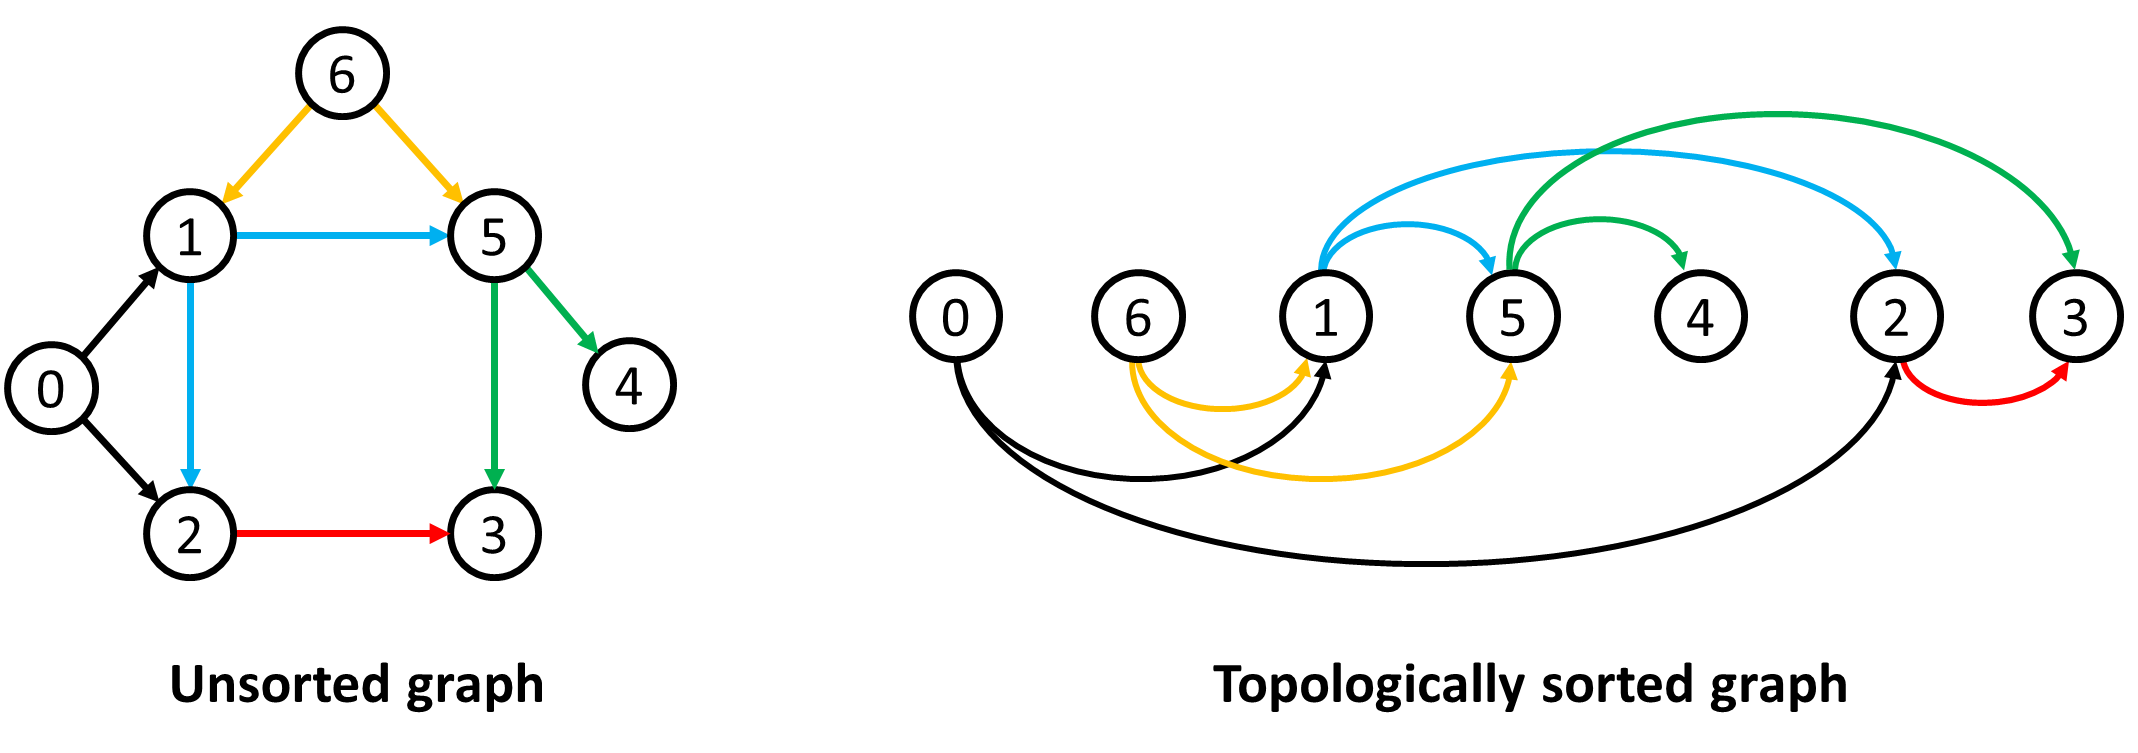
\includegraphics[width=0.6\textwidth]{img/b2/topological_sort_img1.png}
    \caption{Minh họa sắp xếp Tô-pô}
\end{figure}

\subsubsection{Cảm hứng và Động cơ ứng dụng}

Sắp xếp tô-pô là một công cụ quan trọng trong việc mô hình hóa và giải quyết các bài toán liên quan đến \textbf{phụ thuộc thứ tự} giữa các đối tượng. Về bản chất, nó cho phép ta xác định một trình tự thực hiện hợp lệ sao cho mọi điều kiện tiên quyết đều được thỏa mãn trước khi thực hiện bước tiếp theo.

Một ứng dụng thực tế điển hình là trong \textbf{lập kế hoạch công việc}. Khi một tập hợp các công việc có quan hệ phụ thuộc lẫn nhau, ta cần xác định thứ tự thực hiện sao cho mỗi công việc chỉ bắt đầu sau khi tất cả các công việc phụ thuộc của nó đã hoàn thành.

\textbf{Ví dụ minh họa:} Trong chương trình đào tạo đại học, sinh viên cần hoàn thành nhiều học phần để tốt nghiệp. Một số học phần là điều kiện tiên quyết cho các học phần khác. Chẳng hạn:
\begin{itemize}
    \item Để học được môn ``Giới thiệu về thuật toán'', sinh viên phải hoàn thành các môn: ``Nhập môn lập trình'', ``Cấu trúc dữ liệu'', ``Nhập môn thuật toán'', v.v.
\end{itemize}

Ta có thể xây dựng một đồ thị có hướng, trong đó:
\begin{itemize}
    \item Mỗi đỉnh tương ứng với một học phần;
    \item Có một cung từ đỉnh \( u \) đến đỉnh \( v \) nếu học phần \( u \) là điều kiện tiên quyết của học phần \( v \).
\end{itemize}

Khi đó, việc tìm một sắp xếp tô-pô của đồ thị này sẽ cho ta một thứ tự học hợp lệ. Nếu không tồn tại sắp xếp tô-pô (tức đồ thị có chu trình), điều đó phản ánh sự xung đột hoặc vòng lặp trong điều kiện tiên quyết giữa các môn học - một cấu trúc bất hợp lệ trong thiết kế chương trình đào tạo.

\begin{ghichu}
Sắp xếp tô-pô không xử lý các xung đột tài nguyên như trùng lịch học, mà chỉ đảm bảo mối quan hệ thứ tự phụ thuộc.
\end{ghichu}


\begin{ghichu}
Chỉ tồn tại sắp xếp tô-pô nếu và chỉ nếu đồ thị là DAG (Directed Acyclic Graph).

\end{ghichu}


\subsubsection{Chứng minh điều kiện tồn tại thứ tự Tô-pô}

\begin{giathuyet}
    Một đồ thị có hướng tồn tại thứ tự Tô-pô khi và chỉ khi nó là một \textbf{DAG}.
\end{giathuyet}

\begin{giathuyet}
    Đồng nghĩa, mọi DAG đều tồn tại ít nhất một thứ tự Tô-pô.
\end{giathuyet}

\begin{giathuyet}
    Có thể tìm được một thứ tự Tô-pô bằng thuật toán trong thời gian tuyến tính \( \mathcal{O}(V + E) \).
\end{giathuyet}

\begin{chungminh}
Ta sẽ chứng minh hai chiều của giả thuyết chính.

\textbf{Chiều thuận:} Nếu đồ thị \( G \) có chu trình, thì không thể tồn tại thứ tự tô-pô.

Giả sử tồn tại chu trình \( v_1 \to v_2 \to \dots \to v_n \to v_1 \). Khi đó, theo định nghĩa của thứ tự tô-pô, ta có:
\[
\operatorname{order}(v_1) < \operatorname{order}(v_2) < \dots < \operatorname{order}(v_n) < \operatorname{order}(v_1),
\]
tức là \( \operatorname{order}(v_1) < \operatorname{order}(v_1) \), mâu thuẫn. Vậy, nếu có chu trình, không tồn tại thứ tự tô-pô.\\

\textbf{Chiều nghịch:} Nếu \( G \) là một DAG, thì tồn tại ít nhất một thứ tự tô-pô.

\begin{enumerate}
    \item Vì \( G \) không có chu trình, nên tồn tại ít nhất một đỉnh không có cung đi vào (bậc vào bằng 0). Nếu mọi đỉnh đều có bậc vào \(\geq 1\), thì bắt đầu từ một đỉnh bất kỳ, ta luôn đi được sang đỉnh khác (vì có cung đi vào), và cuối cùng sẽ đi thành một chu trình, mâu thuẫn với giả thiết \( G \) là DAG.

    \item Gọi đỉnh đó là \( u \). Đặt \( u \) là đỉnh đầu tiên trong thứ tự tô-pô.

    \item Loại bỏ \( u \) khỏi đồ thị cùng tất cả các cung đi ra từ \( u \). Đồ thị còn lại vẫn là DAG (vì việc xóa đỉnh không thể tạo ra chu trình mới).

    \item Áp dụng lại quá trình trên với đồ thị còn lại: luôn tồn tại đỉnh có bậc vào bằng 0, đưa nó vào tiếp theo trong thứ tự.

    \item Lặp lại cho đến khi tất cả các đỉnh được đưa vào thứ tự.

    \item Cuối cùng, ta thu được một thứ tự thỏa mãn định nghĩa sắp xếp tô-pô.
\end{enumerate}

\begin{figure}[H]
    \centering
    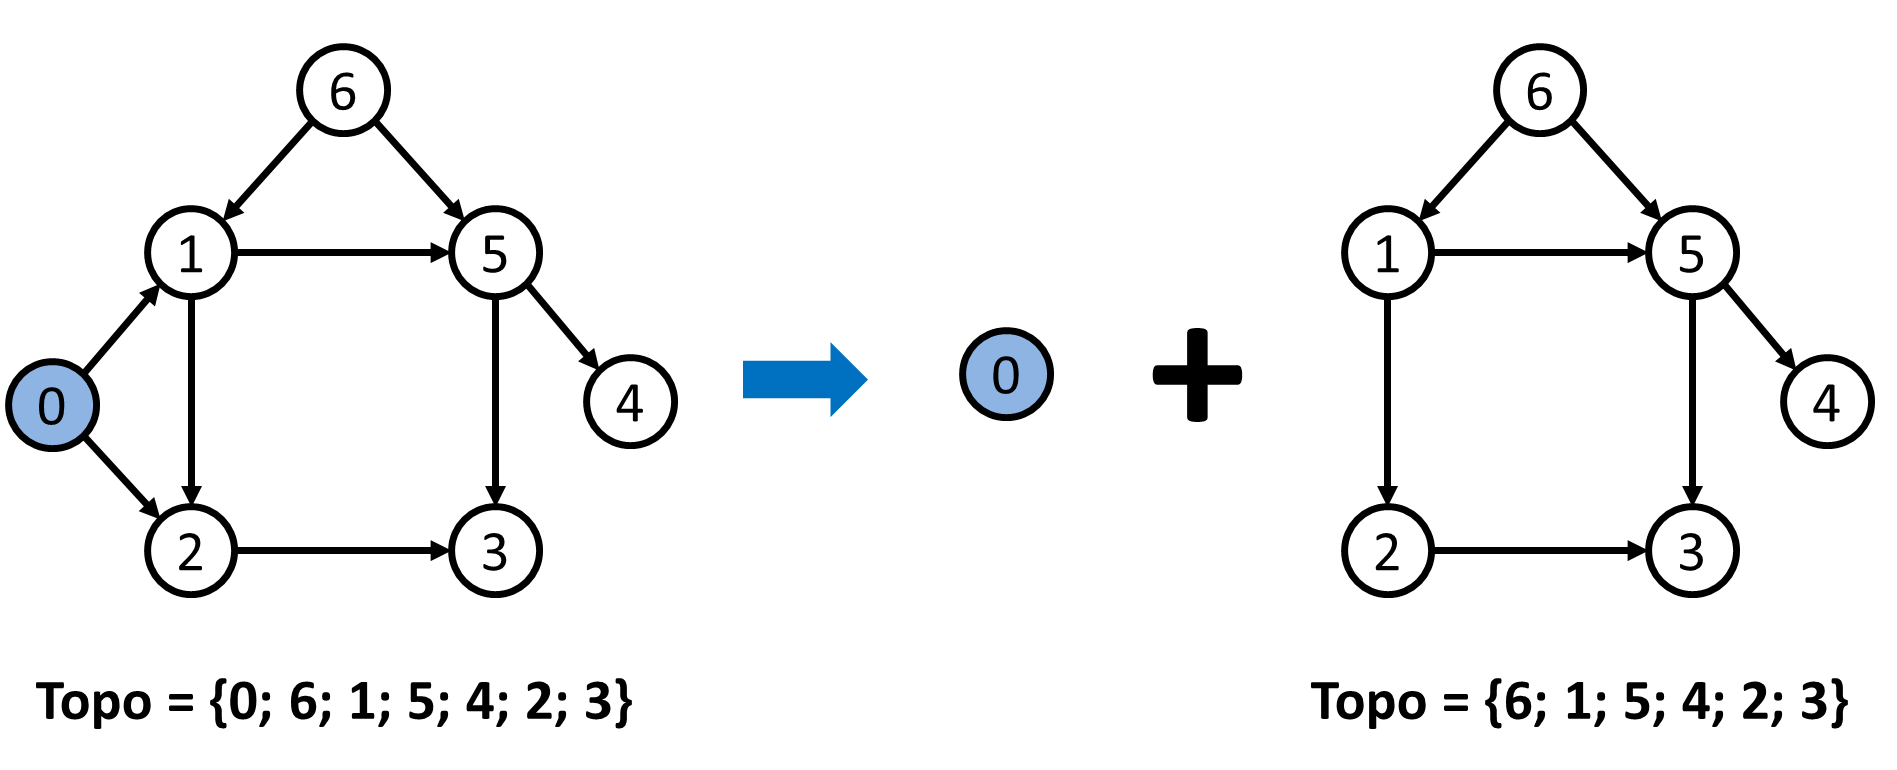
\includegraphics[width=0.6\textwidth]{img/b2/topological_sort_img2.png}
    \caption{Minh họa chứng minh chiều nghịch}
\end{figure}
\textbf{Kết luận:} Với mỗi DAG, luôn tồn tại ít nhất một thứ tự tô-pô.
\end{chungminh}

\subsubsection{Bài tập}
\begin{baitap}
    TOPOSORT - Sắp xếp TOPO
\end{baitap}

\textbf{Đề bài}
Cho đồ thị có hướng không chu trình $G(V, E)$. Hãy đánh số lại các đỉnh của $G$ sao cho chỉ có cung nối từ đỉnh có chỉ số nhỏ đến đỉnh có chỉ số lớn hơn.

\textbf{Input}

\begin{itemize}
    \item Dòng đầu chứa hai số nguyên $n$ $(1 \leq n \leq 100)$ và $m$ $(0 \leq m \leq \frac{n(n-1)}{2})$
    \item $m$ dòng tiếp theo, mỗi dòng chứa một cặp số $u, v$ cho biết một cung nối từ $u \rightarrow v$ trong $G$.
\end{itemize}

\textbf{Output}

Ghi ra $n$ số nguyên dương, số thứ $i$ là chỉ số của đỉnh $i$ sau khi đánh số lại. Hai số trên cùng một dòng được ghi cách nhau một dấu cách (space).

\textbf{Ví dụ}

\begin{lstlisting}[caption={Input}]
7 7
1 2
1 4
2 3
4 5
6 5
5 3
7 4 
\end{lstlisting}

\begin{lstlisting}[caption={Output}]
1 2 7 5 6 3 4
\end{lstlisting}

\begin{figure}[H]
    \centering
    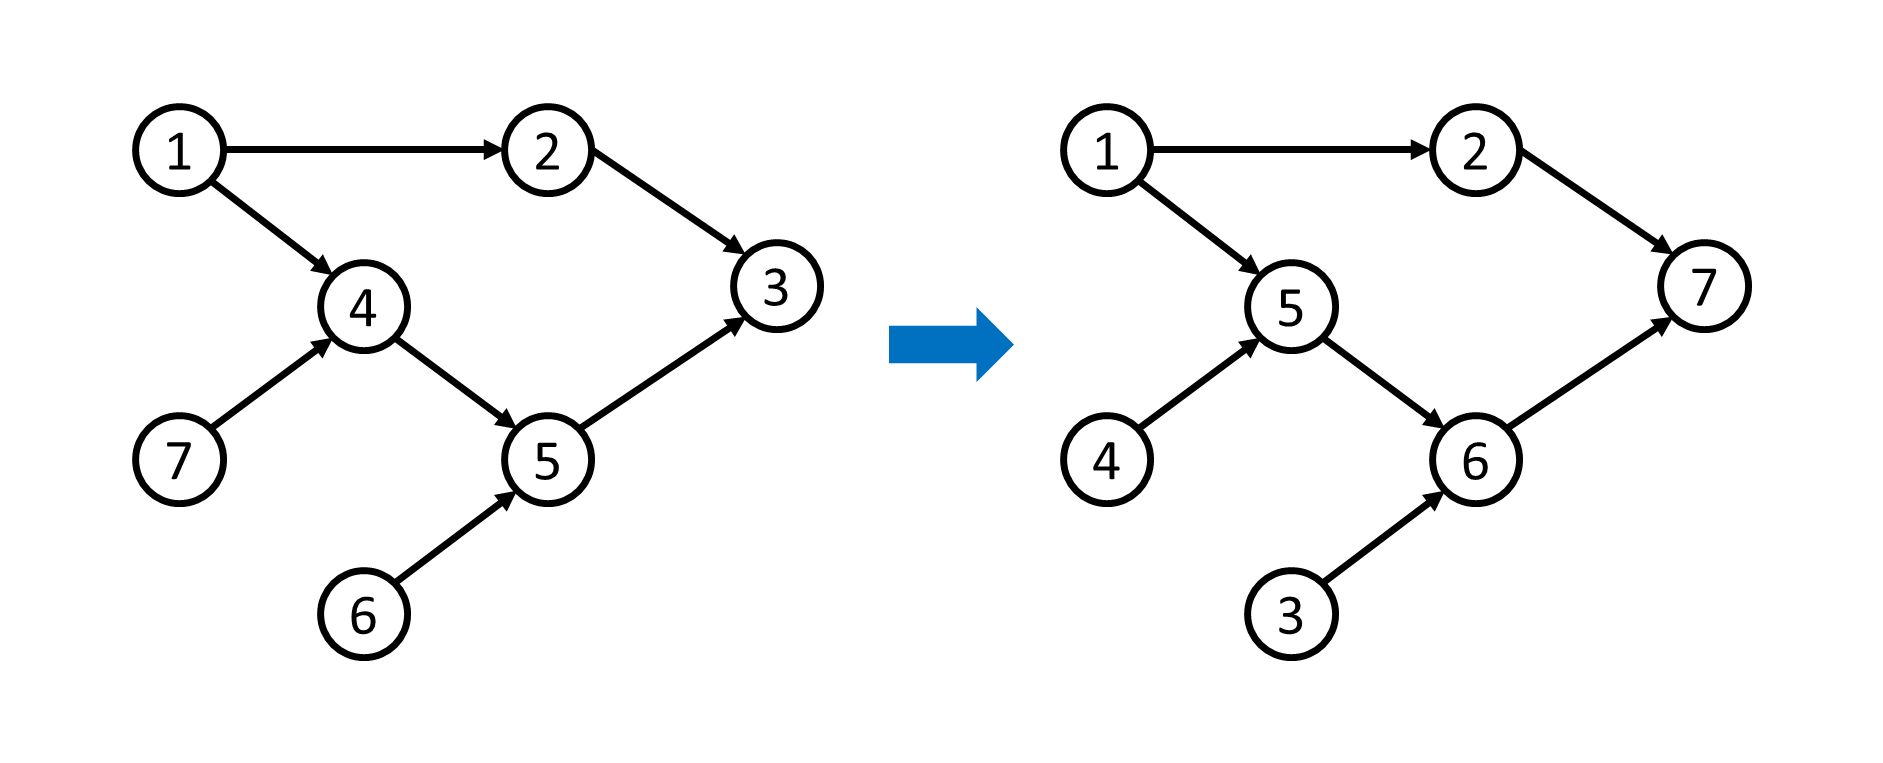
\includegraphics[width=0.6\textwidth]{img/b2/topological_sort_img3.png}
    \caption{Minh họa ví dụ}
\end{figure}

\textbf{Phân tích bài toán}

Với một đỉnh $u$ bất kỳ, khi DFS thăm đến một đỉnh u, sau khi đã đệ quy thăm hết tất cả các đỉnh con của nó, ta đẩy u vào ngăn xếp (\href{https://wiki.vnoi.info/algo/data-structures/Stack}{Stack}). Lúc này ngăn xếp sẽ chứa các đỉnh theo thứ tự ``postorder'' đảo ngược (reverse postorder) -- postorder là thời điểm kết thúc của DFS tại đỉnh đó. 

Để gán nhãn, ta lấy lần lượt từng đỉnh trên cùng của ngăn xếp (tương đương là đỉnh có postorder muộn nhất), gán nhãn lần lượt $1, 2, \dots, n$ đến khi ngăn xếp rỗng (đã xử lý hết đỉnh). Ta đảm bảo được rằng, nếu $u$ được đẩy trước $v$ (tức là hoàn thành DFS sớm hơn), thì $u$ sẽ được gán nhãn lớn hơn.

\begin{lstlisting}[language=C++, caption={Cài đặt Sắp xếp Tô-pô bằng DFS}, label={code:toposort}]
    #include <bits/stdc++.h>
#define int long long
#define endl "\n"
using namespace std;

int n, m;
vector<int> adj[101];
stack<int> st;
vector<bool> visited(101, false);

void dfs(int u) {
    visited[u] = true;
    for (auto v : adj[u]) {
        if (visited[v] == false) {
            dfs(v);
        }
    }
    st.push(u);
}

signed main() {
    cin >> n >> m;
    for (int i = 1; i <= m; i++) {
        int u, v; cin >> u >> v;
        adj[u].push_back(v);
    }    
    for (int i = 1; i <= n; i++) {
        if (visited[i] == false) {
            dfs(i);
        }
    }
    vector<int> ans(n + 1, 0);
    int cnt = 1;
    while (st.empty() == false) {
        ans[st.top()] = cnt++;
        st.pop();
    }
    for (int i = 1; i <= n; i++) {
        cout << ans[i] << " ";
    }
    return 0;
}

\end{lstlisting}

\begin{baitap}
    \href{https://cses.fi/problemset/task/1679}{Course Schedule}
\end{baitap}

\textbf{Đề bài}

Cho $n$ khóa học, có $m$ yêu cầu có dạng ``khóa học $a$ phải được hoàn thành mới đủ điều kiện học khóa học $b$''. Nhiệm vụ của bạn là tìm thứ tự học sao cho hoàn thành toàn bộ khóa học.

\textbf{Input}

\begin{itemize}
    \item Dòng đầu tiên chứa 2 số nguyên $n$ $(1 \leq n \leq 10^5)$ và $m$ $(1 \leq m \leq 2.10^5)$
    \item $m$ dòng tiếp theo mô tả các yêu cầu. Mỗi dòng chứa hai số nguyên $a$ và $b$ $(1 \leq a, b \leq n)$: khóa học $a$ phải được hoàn thành trước khóa học $b$.
\end{itemize}

\textbf{Output}

In ra thứ tự học để hoàn thành các khóa học. Có thể in bất kỳ thứ tự nào thỏa mãn. 

Nếu không tìm được thứ tự thỏa mãn, in ra ``IMPOSSIBLE''.

\textbf{Ví dụ}

\begin{lstlisting}[caption={Input}]
5 3
1 2
3 1
4 5
\end{lstlisting}

\begin{lstlisting}[caption={Output}]
4 5 3 1 2
\end{lstlisting}

\textbf{Phân tích bài toán}

Để tìm được thứ tự thỏa mãn, ta phải đảm bảo rằng đồ thị biểu diễn là một DAG. 

Để kiểm tra đồ thị có phải là DAG, ta kiểm tra như sau:
\begin{itemize}
    \item Gọi mảng kiểm tra trạng thái duyệt của đỉnh $i$ bất kỳ là visited[i] = {0, 1, 2} với ý nghĩa lần lượt là: chưa thăm, đang thăm, đã thăm xong.
    \item Khi duyệt đỉnh $u$, đặt trạng thái visited[u] = 1.
    \item Thăm các con $v_i$ của $u$, nếu tồn tại $v_i$ đang có trạng thái visited[$v_i$] = 1, nghĩa là đồ thị có chu trình $\rightarrow$ Không phải là DAG, ta in ra ``IMPOSSIBLE''.
    \item Ngược lại, nếu visited[$v_i$] = 0, ta thăm $v_i$.
    \item Sau khi thăm xong, ta đặt trạng thái visited[u] = 2. 
\end{itemize}

Phần tìm thứ tự là một bài toán Sắp xếp Tô-pô, đã được mô tả thuật toán ở bài \textbf{TOPOSORT - Sắp xếp TOPO} phía trên.

\begin{lstlisting}[language=C++, caption={Cài đặt}, label={code:CourseSchedule}]
#include <bits/stdc++.h>
#define int long long
#define endl "\n"
using namespace std;

vector<int> adj[100005];
int n, m; 
vector<int> visited(100005, 0);
stack<int> st;
void dfs(int u) {
    visited[u] = 1;
    for (auto v : adj[u]) {
        if (visited[v] == 1) {
            cout << "IMPOSSIBLE";
            exit(0);
        }
        if (visited[v] == 0) dfs(v);
    }
    visited[u] = 2;
    st.push(u);
}
signed main() {
    cin >> n >> m;
    for (int i = 1; i <= m; i++) {
        int u, v; cin >> u >> v;
        adj[u].push_back(v);
    }    
    for (int i = 1; i <= n; i++) {
        if (visited[i] == 0) {
            dfs(i);
        }
    }
    while (st.empty() == false) {
        cout << st.top() << " ";
        st.pop();
    }
    return 0;
}
\end{lstlisting}


\begin{baitap}
    \href{https://atcoder.jp/contests/dp/tasks/dp_g}{Longest Path}
\end{baitap}

\textbf{Đề bài}

Cho đồ thị $G$ với $N$ đỉnh và $M$ cạnh. $G$ không tồn tại chu trình có hướng. \\

Hãy tìm độ dài của đường đi có hướng dài nhất trong đồ thị $G$. Độ dài đường đi có hướng dài nhất là tổng số cạnh có trong đường đi đó.

\textbf{Input}

\begin{itemize}
    \item Dòng đầu tiên chứa 2 số nguyên $N$ $(1 \leq n \leq 10^5)$ và $M$ $(1 \leq m \leq 10^5)$
    \item $M$ dòng tiếp theo mô tả các yêu cầu. Mỗi dòng chứa hai số nguyên $x$ và $y$ $(1 \leq x, y \leq n)$ với ý nghĩa: tồn tại cạnh có hướng từ đỉnh $x \rightarrow y$.
\end{itemize}

\textbf{Output}

In ra độ dài đường đi có hướng dài nhất trong đồ thị $G$.

\textbf{Ví dụ}
\begin{lstlisting}[caption={Input}]
4 5
1 2
1 3
3 2
2 4
3 4
\end{lstlisting}

\begin{lstlisting}[caption={Output}]
3
\end{lstlisting}

\begin{figure}[h]
    \centering
    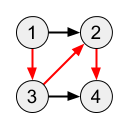
\includegraphics[width=0.1 \textwidth]{img/b2/longest_0_muffet.png}
    \caption{Mô tả ví dụ}    
\end{figure}

\textbf{Phân tích bài toán}

Gọi $dp[u]$ là đường đi có hướng dài nhất kết thúc tại đỉnh $u$. Với $dp[i] = 0, \forall i \in [1..N]$. 

Giả sử đã biết được giá trị $dp[u]$, với mỗi cạnh có hướng từ $u \rightarrow v$, ta cập nhật được:
\[
    dp[v] = \max(dp[v], dp[u] + 1)
\]

Với ý nghĩa là nếu ta đi từ $u \rightarrow v$, thì đường đi có hướng dài nhất kết thúc ở $v$ có thể thu được bằng đường đi có hướng dài nhất đến $u$ cộng thêm 1 bước.

Để đảm bảo mỗi khi cập nhật dp[v] thì dp[u] đã được tính xong, ta duyệt các đỉnh theo thứ tự tô-pô của đồ thị.\\

Như vậy, sau khi lặp qua hết các cạnh theo thứ tự tô-pô, giá trị $\max_{1 \leq i \leq N} dp[i]$ chính là độ dài đường đi có hướng dài nhất trong toàn đồ thị.\\

\textbf{Câu hỏi phụ:} Tại sao với $dp[v]$ cần lấy $\max(dp[v], dp[u] + 1)$?

\textbf{Trả lời luôn:} Vì trước khi thăm $v$ từ đỉnh $u$, có thể tồn tại đường đi dài nhất kết thúc tại $v$ mà không thông qua đỉnh $u$. Vì vậy ta cần lấy $\max$ của 2 trường hợp: tồn tại đường đi dài nhất kết thúc tại $v$ mà: không qua $u$ $\&$ qua $u$.\\

\textbf{Ngoài lề:} Vì tác giả lười xử lý/thao tác trên ngăn xếp (stack) nên sau này với các bài toán sắp xếp tô-pô, tác giả sẽ thao tác trên vector và reverse vector để lấy thứ tự tô-pô (Vector is the best data structure in C++/the world).

\begin{lstlisting}[language=C++, caption={Cài đặt}, label={code:CourseSchedule}]
#include <bits/stdc++.h>
#define int long long
#define endl "\n"
using namespace std;

vector<int> adj[100005];
int n, m; 
vector<int> visited(100005, 0);
vector<int> dp(100005, 0);
vector<int> st;

void dfs(int u) {
    visited[u] = true;
    for (auto v : adj[u]) {
        if (!visited[v]) dfs(v);
    }
    st.push_back(u);
}

signed main() {
    cin >> n >> m;
    for (int i = 1; i <= m; i++) {
        int u, v; cin >> u >> v;
        adj[u].push_back(v);
    }    

    for (int i = 1; i <= n; i++) {
        if (visited[i] == false) {
            dfs(i);
        }
    }
    reverse(st.begin(), st.end());

    for (auto u : st) {
        for (auto v : adj[u]) {
            dp[v] = dp[u] + 1;
        }
    }
    int ans = 0;
    for (int i = 1; i <= n; i++) ans = max(ans, dp[i]);
    cout << ans;
    return 0;
}
\end{lstlisting}

\subsection{Cây DFS (Depth-First Search Tree) và ứng dụng}
Nội dung bài chủ yếu tham khảo/copy từ [VNOI WIKI]: \url{https://wiki.vnoi.info/algo/graph-theory/Depth-First-Search-Tree.md}

\subsubsection{Cây duyệt chiều sâu DFS (cây DFS)}

Trong quá trình $DFS$, với mỗi đỉnh $u$ ta có $par[u]$ là số hiệu của đỉnh mà từ đỉnh đó thủ tục $DFS$ gọi để quy đến $u$. Xây dựng đồ thị con với các cạnh là $(par[u], u)$, ta có được một cây. Cây này được gọi là \textbf{cây $DFS$}.   

Các cạnh thuộc cây $DFS$ được gọi là các ``cạnh nét liền''.

Các cạnh còn lại không thuộc cây $DFS$ được gọi là các ``cạnh nét đứt''.\\

Nói cách khác, khi ta thực hiện $DFS$, tưởng tượng như sau:

\begin{enumerate}
    \item Bắt đầu từ một đỉnh gốc:

    – Ta gọi DFS tại đó, coi nó là “gốc” của cây.
    \item Mỗi lần đi từ u xuống v lần đầu tiên
    
    – Nếu v chưa được thăm, ta đánh dấu par[v] = u (vì u ``gọi'' v), và gọi tiếp DFS(v).
    
    – Cạnh (u, v) đó chính là một cạnh cây (nét liền), vì nó nằm trên hành trình ta thực sự đi.
    \item Khi gặp một cạnh nối u với một đỉnh v đã thăm rồi
    
    – Ta không đi tiếp, vì v đã vào cây.

    – Cạnh đó được gọi là cạnh không phải cây (nét đứt). Nó chỉ là ``đường tắt'' giữa hai đỉnh đã có trong cây.
\end{enumerate}


\begin{figure}[h]
    \centering
    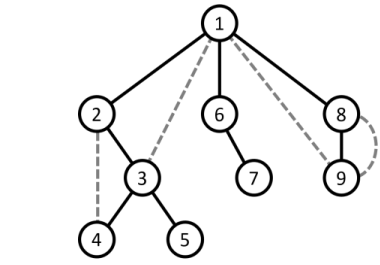
\includegraphics[width=0.3\textwidth]{img/b3/Depth-First-Search-Tree_img1.png}
    \caption{Minh họa cây DFS}    
\end{figure}

Trong đồ thị có hướng, xét các cung được thăm và không được thăm bởi $DFS$, ta có 4 loại cung sau:
\begin{itemize}
    \item Cung của cây $DFS$ \textbf{(Tree egde):} là các cung thuộc cây $DFS$ được định hướng theo chiều từ cha đến con. (ví dụ cạnh $(u, v)$ thuộc cây $DFS$ mà $u$ được thăm trước $v$ hay $u$ là cha của $v$ thì ta có cung $u \rightarrow v$ là cung của cây $DFS$). < Các cung của cây $DFS$ được đánh dấu là các cạnh màu đen trong hình bên dưới >
    \item Cung xuôi \textbf{(Forward edge):} là các cung không thuộc cây $DFS$ và có dạng $u \rightarrow v$ trong đó $u$ là tổ tiên của $v$ trong cây $DFS$. < Các cung xuôi được đánh dấu là các cạnh màu xanh lá trong hình bên dưới >
    \item Cung ngược \textbf{(Back edge):} là các cung không thuộc cây $DFS$ và có dạng $v \rightarrow u$ trong đó $u$ là tổ tiên của $v$ trong cây $DFS$. < Các cung ngược được đánh dấu là các cạnh màu đỏ trong hình bên dưới >
    \item Cung chéo \textbf{(Cross edge):} là các cung không thuộc cây $DFS$ và có dạng $u \rightarrow v$ trong đó $u$ và $v$ thuộc hai nhánh khác nhau của cùng một cây $DFS$. < Các cung chéo được đánh dấu là các cạnh màu xanh dương trong hình bên dưới >
\end{itemize}

\begin{figure}[h]
    \centering
    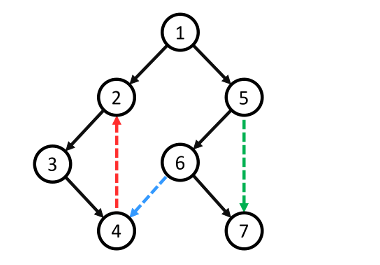
\includegraphics[width=0.2\textwidth]{img/b3/Depth-First-Search-Tree_img2.png}   
    \caption{Mô tả các loại cung trong cây} 
\end{figure}


Trong đồ thị vô hướng:
\begin{itemize}
    \item Không tồn tại cung chéo. Vì khi đỉnh $u$ được duyệt trong hàm $DFS$ ta sẽ duyệt tất cả các đỉnh $v$ kề $u$ mà $v$ chưa được thăm. Như vậy nếu tồn tại một cung chéo $(u, v)$ chứng tỏ khi duyệt đến đỉnh $u$ hoặc đỉnh $v$ ta đã không duyệt cạnh $(u, v)$.
    \item Vì các cạnh trên đồ thị vô hướng không được định chiều nên không thể định nghĩa 2 loại cung xuôi và cung ngược như ở đồ thị có hướng. Do đó, ở đồ thị vô hướng, cung xuôi và cung ngược sẽ được định nghĩa như sau:
    \begin{itemize}
        \item Cung xuôi \textbf{(Forward edge):} là các cung thuộc cây $DFS$. Hay còn có cách gọi khác là ``cạnh nét liền'' hoặc ``cung của cây $DFS$''.
        \item Cung ngược (Back edge): là các cung không thuộc cây $DFS$. Hay còn có cách gọi khác là ``cạnh nét đứt''.
    \end{itemize}
    \item Như vậy trên đồ thị vô hướng lúc này chỉ còn  loại cung là cung ngược và cung xuôi (cung của cây $DFS$).
\end{itemize}

\textbf{Một số mảng quan trọng trong cây DFS:}

\begin{itemize}
    \item Mảng \textbf{num[]}: cho biết thứ tự duyệt DFS của các đỉnh (thứ tự mà mỗi đỉnh bắt đầu duyệt).
    \item Mảng \textbf{low[]}: Với mỗi đỉnh $u$, $low[u]$ cho biết thứ tự (giá trị $num$) nhỏ nhất có thể đi đến được từ $u$ bằng cách đi xuôi xuống theo các cạnh nét liền (các cung trên cây DFS) và kết thúc đi ngược lên không quá 1 lần theo cạnh nét đứt. Ngoài ra ta cũng có thể hiểu ý nghĩa của $low[u]$ là thứ tự thăm của đỉnh có thứ tự thăm sớm nhất nằm trong cây con gốc $u$ hoặc kề cạnh với 1 đỉnh bất kì nằm trong cây con gốc $u$.
    \item Mảng \textbf{tail[]}: cho biết thời điểm kết thúc duyệt DFS của mỗi đỉnh cũng là thời điểm duyệt xong của đỉnh đó.
\end{itemize}

\noindent\textbf{Nhận xét:} Các đỉnh có thứ tự thăm nằm trong khoảng từ $num[u]$ đến $tail[u]$ chính là các đỉnh nằm trong cây con gốc $u$ trong cây DFS.\\

\textbf{Cách tính mảng low[], num[], tail[]:}

\begin{itemize}
    \item \textbf{Ý tưởng chính:} Mảng $num[]$, $tail[]$ ta có thể tính dễ dàng bằng cách DFS xác định thời điểm duyệt tới và thời điểm duyệt xong của các đỉnh. Với mảng $low[]$ ta có:
    \begin{itemize}
        \item Trước hết, với 1 đỉnh $u$ bất kì có thể tự đi tới chính nó nên ta gán $low[u] = num[u]$.
        \item Từ $u$ có thể đến các đỉnh $v$ kề u bằng 1 cạnh nét đứt nên ta có $low[u] = \min(low[u], num[v])$ với $(u, v)$ là một cạnh nét đứt.
        \item Ngược lại, nếu $(u, v)$ là một cạnh nét liền và v không phải cha của u ta có $low[u] = \min(low[u], low[v])$ do từ $u$ ta có thể đi xuống $v$ sau đó đi theo con đường đã xác định ở đỉnh $v$ để tới đỉnh có thứ tự thăm là $low[v]$.
    \end{itemize}
    \item \textbf{Chú ý:} Giá trị thực sự của $num[], low[]$ được xác định bằng giá trị thực sự của $low[u], tail[u]$ chỉ được xác định khi đã duyệt xong đỉnh $u$. Thời điểm duyệt tới của một đỉnh $u$ luôn diễn ra trước thời điểm duyệt tới của các đỉnh trong cây con gốc $u$ của cây DFS, thời điểm duyệt xong của đỉnh $u$ luôn diễn ra sau thời điểm duyệt xong của các đỉnh trong cây con gốc $u$.

    \item \textbf{Cách thực hiện:}
    \begin{itemize}
        \item Đầu tiên ta sẽ bắt đầu duyệt $DFS$ từ đỉnh gốc. Khi duyệt tới đỉnh $u$ ta sẽ cập nhật thời điểm duyệt tới. Lúc này $low[u] = num[u] =$ \textit{thứ tự duyệt DFS}. Ta sẽ duyệt tất cả các con $v$ trong gốc $u$.
        \item \textbf{Trường hợp 1:} Nếu đỉnh $v$ chưa được thăm thì sau khi hoàn thành $DFS$ của $v$ thì ta sẽ cập nhật lại giá trị của $low[u]$: $low[u] = \min(low[u], low[v])$;
        \item \textbf{Trường hợp 2:} Nếu đỉnh $v$ đã được thăm, thì ta sẽ cập nhật lại giá trị cho $low[u]$: $low[u] = \min(low[u], num[v])$;
        \item Ở trường hợp này ta không thể cập nhật $low[u] = \min(low[u], low[v])$ được. Vì khi ta thăm đến đỉnh $u$ mà đỉnh $v$ đã được thăm thì tức là $(u, v)$ là một cạnh nét đứt, do đó khi đi từ $u$ ta đã sử dụng 1 cạnh nét đứt nên không thể tiếp tục di chuyển nữa (theo định nghĩa của mảng $low[]$) suy ra ta chỉ cập nhật $low[u] = \min(low[u], num[v])$.
    \end{itemize}
    \item \textbf{Chú ý:} \textit{Nếu v là cha trực tiếp của u thì ta bỏ qua không xét đến.}
    \item Khi đã duyệt xong đỉnh $u$ và các nút trong cây con $DFS$ gốc $u$ ta sẽ tiến hành cập nhật giá trị $tail[u] =$ \textit{thời gian duyệt DFS hiện tại}.
\end{itemize}

\begin{lstlisting}[language=C++, caption={Cài đặt}]
int timeDfs = 0; 

void dfs(int u, int pre) {
    num[u] = low[u] = ++timeDfs;
    for (int v : g[u]){
        if (v == pre) continue;
        if (!num[v]) {
            dfs(v, u);
            low[u] = min(low[u], low[v]);
        }
        else low[u] = min(low[u], num[v]);
    }
    tail[u] = timeDfs;
}
\end{lstlisting}

\begin{figure}[h]
    \centering
    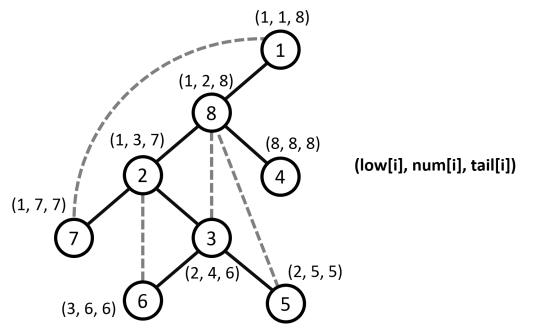
\includegraphics[width=0.4\textwidth]{img/b3/Depth-First-Search-Tree_img3.png}  
    \caption{Ví dụ minh họa}  
\end{figure}

\subsection{Khớp và Cầu (Joints and Brides)}
\begin{dinhnghia}
    
    \item Trong đồ thị vô hướng, một đỉnh được gọi là đỉnh khớp nếu như loại bỏ đỉnh này và các cạnh liên thuộc với nó ra khỏi đồ thị thì số thành phần liên thông của đồ thị tăng lên.
    
    \item Trong đồ thị vô hướng, một cạnh được gọi là cạnh cầu nếu như loại bỏ cạnh này ra khỏi đồ thị thì số thành phần liên thông của đồ thị tăng lên.
\end{dinhnghia}

\begin{figure}[h]
    \centering
    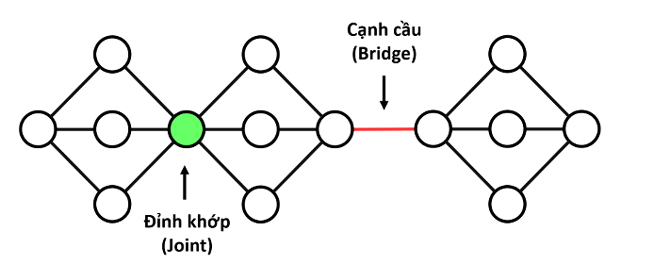
\includegraphics[width=0.5\textwidth]{img/b4/Depth-First-Search-Tree_img4.png}   
    \caption{Minh họa khớp và cầu} 
\end{figure}

\begin{baitap}
    \href{https://oj.vnoi.info/problem/graph_}{GRAPH\_ - Tìm khớp và cầu (Cơ bản)}
\end{baitap}

Xét đơn đồ thị vô hướng $G = (V, E)$ có $N$ ($1 \leq N \leq 10000$) đỉnh và $M$ ($1 \leq M \leq 50000$) cạnh. Người ta định nghĩa một đỉnh gọi là khớp nếu như xóa đỉnh đó sẽ làm tăng số thành phần liên thông của đồ thị. Tương tự như vậy, một cạnh được gọi là cầu nếu xóa cạnh đó sẽ làm tăng số thành phần liên thông của đồ thị.

Vấn đề đặt ra là cần đếm tất cả các khớp và cầu của đồ thị $G$.

\textbf{Input}
\begin{itemize}
    \item Dòng đầu: chứa hai số tự nhiên $N$, $M$.
    \item $M$ dòng sau, mỗi dòng chứa một cặp số $(u, v)$ ($u \neq v$, $1 \leq u \leq N, 1 \leq v \leq N$) mô tả một cạnh của $G$.
\end{itemize}

\textbf{Output}
\begin{itemize}
    \item Gồm một dòng duy nhất ghi hai số, số thứ nhất là số khớp, số thứ hai là số cầu của $G$.
\end{itemize}

\textbf{Example}

\begin{lstlisting}[caption={Input}]
10 12
1 10
10 2
10 3
2 4
4 5
5 2
3 6
6 7
7 3
7 8
8 9
9 7
\end{lstlisting}
\begin{lstlisting}[caption={Output}]
4 3 
\end{lstlisting}

\textbf{Note}
\begin{itemize}
    \item Các cạnh màu đỏ là cạnh cầu.
    \item Các đỉnh màu xanh lá là đỉnh khớp.
\end{itemize}

\begin{figure}[h]
    \centering
    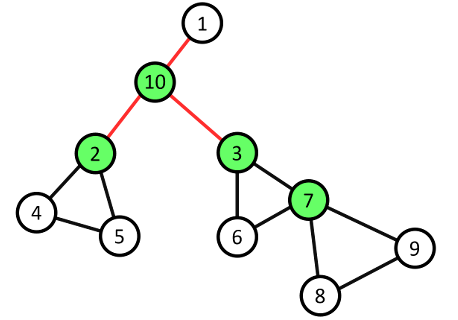
\includegraphics[width=0.3\textwidth]{img/b4/Depth-First-Search-Tree_img5.png}
    \caption{Minh họa ví dụ}
\end{figure}

\subsubsection*{Phân tích}

\textbf{Tìm cạnh cầu}
\begin{itemize}
    \item Dễ thấy rằng cạnh cầu của đồ thị không thể là cạnh nét đứt vì việc bỏ đi cạnh nét đứt sẽ không ảnh hưởng đến tính liên thông giữa các đỉnh của đồ thị. Do vậy, cạnh cầu chỉ có thể là cạnh nét liền.
    \item Ta sẽ xét riêng từng thành phần liên thông của đồ thị. Xét vùng liên thông $G$ như sau:
    \begin{itemize}
        \item Xét cây con gốc $v$ trong cây $DFS$ của $G$ có $u$ là cha trực tiếp của $v$. Gọi tập hợp các đỉnh thuộc cây con gốc $v$ là $A$, tập hợp các đỉnh không thuộc cây con gốc $v$ là $B$. Khi xóa đi cạnh $(u, v)$ thì giữa 2 đỉnh bất kì thuộc cùng 1 tập hợp vẫn có thể đến với nhau bằng các cạnh nét liền. Một đỉnh thuộc $A$ với một đỉnh thuộc $B$ muốn đi đến với nhau bằng các \textbf{cạnh nét liền} thì đều phải thông qua cạnh $(u, v)$.
        \item \textbf{Ví dụ minh họa:} Xét cạnh nét liền $(7, 9)$ với đỉnh $9$ là con trực tiếp của đỉnh $7$ trên cây $DFS$. Tập đỉnh $A$ là các đỉnh được đánh dấu màu hồng. Tập đỉnh $B$ là các đỉnh được đánh dấu màu vàng. Đỉnh $11$ thuộc tập $A$ muốn đi đến đỉnh $6$ thuộc tập $B$ bằng các cạnh nét liền thì đều phải thông qua cạnh $(7, 9)$.
    \end{itemize}
\end{itemize}

\begin{figure}[h]
    \centering
    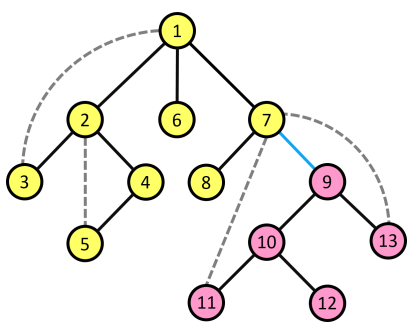
\includegraphics[width=0.3\textwidth]{img/b4/Depth-First-Search-Tree_img6.png}
\end{figure}

\begin{itemize}
    \item Giả sử không có cạnh nét đứt nào nối giữa 1 đỉnh thuộc $A$ với 1 đỉnh thuộc $B$ thì khi xóa cạnh $(u, v)$, $G$ sẽ tách ra thành 2 vùng liên thông $A$ và $B$. Ngược lại nếu tồn tại cạnh nét đứt nối giữa 1 đỉnh thuộc $A$ và 1 đỉnh thuộc $B$ đồ thị vẫn liên thông. Do đó ta chỉ cần xét xem có tồn tại cạnh nét đứt nối giữa $A$ và $B$ hay không để kết luận $(u, v)$ có phải cầu không?
    \item Ta có từ $v$ có thể đi đến một đỉnh $p$ nào đó có $num[p] = low[v]$ bằng cách đi theo các cung của cây $DFS$ và đi qua không quá 1 cạnh nét đứt và $p$ có thứ tự thăm sớm nhất khi $DFS$. Nếu $p$ nằm trong $B$ thì $p$ phải là tổ tiên của $v$ cũng đồng nghĩa với việc $num[p] < num[v]$ hay $low[v] < num[v]$ (\textbf{vì đồ thị không có cung chéo}), nghĩa là tồn tại 1 cạnh nét đứt nối giữa 1 đỉnh thuộc $A$ với 1 đỉnh thuộc $B$ (vì nếu chỉ đi bằng các cung của cây $DFS$ thì $v$ không thể tới một tổ tiên của nó).
    \item Do đó nếu $low[v] \geq num[v]$ chắc chắn đỉnh $p$ thuộc cây con gốc $v$ hay $p$ thuộc tập hợp $A$ khi đó không tồn tại cạnh nét đứt nối giữa 1 đỉnh thuộc $A$ với 1 đỉnh thuộc $B$. Tuy nhiên, ta dễ dàng nhận thấy $low[v] \leq num[v]$ vì đỉnh $v$ luôn tới được chính nó.
\end{itemize}

\noindent\textbf{Kết luận:} Nếu $low[v] = num[v]$ thì $(u, v)$ là một cạnh cầu trong đồ thị.

\textbf{Tìm đỉnh khớp}
\begin{itemize}
    \item Ta sẽ xét riêng từng thành phần liên thông của đồ thị. Xét vùng liên thông $G$ như sau:
    \begin{itemize}
        \item Xét cây con gốc $u$ trong cây $DFS$ của $G$, nếu mọi nhánh con của $u$ đều có cung ngược lên tới tổ tiên của $u$ ($low[v] < num[u]$, với $v$ là tất cả các con trực tiếp của $u$ trên cây $DFS$) thì đỉnh $u$ không thể là đỉnh khớp. Bởi trong đồ thị ban đầu, nếu ta loại bỏ đỉnh $u$ đi thì từ mỗi đỉnh bất kỳ thuộc nhánh con vẫn có thể đi lên một tổ tiên của $u$, rồi đi sang nhánh con khác hoặc đi sang tất cả những đỉnh còn lại của cây nên số thành phần liên thông của đồ thị không thay đổi.
        \item \textbf{Ví dụ minh họa:} Xét đỉnh $9$ không phải là đỉnh khớp vì cả 2 nhánh con của nó là cây con gốc $10$ và cây con gốc $13$ trong cây $DFS$ đều có cung ngược lên tới đỉnh $7$ là tổ tiên của đỉnh $9$.
    \end{itemize}
\end{itemize}
\begin{figure}[h]   
    \centering
    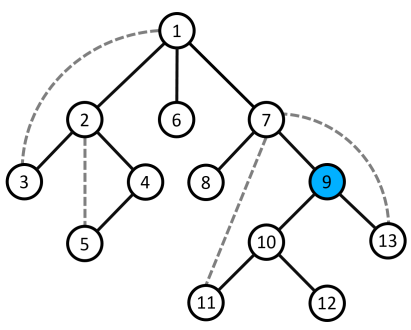
\includegraphics[width=0.3\textwidth]{img/b4/Depth-First-Search-Tree_img7.png}
\end{figure}

\begin{itemize}
    \item Nếu $u$ không phải là đỉnh gốc của cây $DFS$, và tồn tại ít nhất một nhánh con trong cây con gốc $u$ không có cung ngược lên một tổ tiên của $u$ ($low[v] \geq num[u]$, với $v$ là một con trực tiếp bất kì của $u$ trên cây $DFS$) thì đỉnh $u$ là đỉnh khớp. Bởi khi đó, tất cả những cung xuất phát từ nhánh con đó chỉ có thể đi tới những đỉnh thuộc cây con gốc $u$ mà thôi, trên đồ thị ban đầu, không tồn tại cạnh nối từ những đỉnh thuộc nhánh con đó tới một tổ tiên của $u$. Vậy nên từ một đỉnh bất kì thuộc nhánh con đó muốn đi lên một tổ tiên của $u$ thì bắt buộc phải đi qua $u$ nên việc loại bỏ đỉnh $u$ ra khỏi đồ thị sẽ làm tăng số thành phần liên thông của đồ thị.
    \item \textbf{Ví dụ minh họa:} Xét đỉnh $2$ là đỉnh khớp vì tồn tại 1 nhánh con của nó là cây con gốc $4$ không có cung ngược lên tới tổ tiên của đỉnh $2$.
\end{itemize}

\begin{figure}[h]   
    \centering
    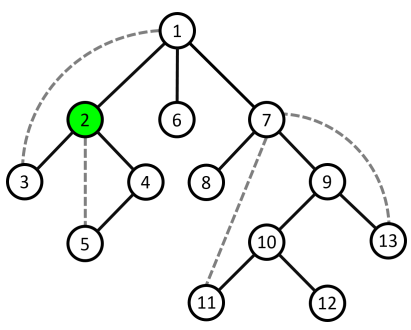
\includegraphics[width=0.3\textwidth]{img/b4/Depth-First-Search-Tree_img8.png}
\end{figure}

\begin{itemize}
    \item Nếu $u$ là đỉnh gốc của cây $DFS$, thì $u$ là đỉnh khớp khi và chỉ khi $u$ có ít nhất 2 nhánh con. Vì đồ thị không có cung chéo nên khi $u$ có 2 nhánh con thì đường đi giữa hai đỉnh thuộc hai nhánh con đó bắt buộc phải đi qua $u$. Việc loại bỏ đỉnh $u$ ra khỏi đồ thị sẽ làm tăng số thành phần liên thông của đồ thị.
    \item \textbf{Ví dụ minh họa:} Xét đỉnh $1$ là đỉnh khớp vì đỉnh $1$ là đỉnh gốc của cây $DFS$ và có tới $3$ nhánh con.
\end{itemize}

\begin{figure}[h]   
    \centering
    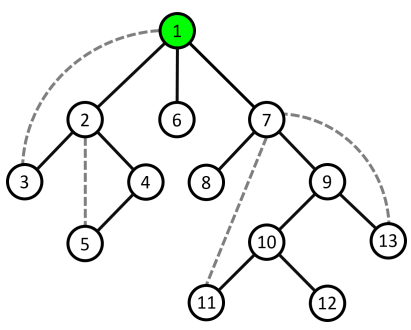
\includegraphics[width=0.3\textwidth]{img/b4/Depth-First-Search-Tree_img9.png}
\end{figure}

\textbf{Kết luận:} Đỉnh $u$ là đỉnh khớp khi:
\begin{itemize}
    \item Đỉnh $u$ không phải là gốc của cây $DFS$ và $low[v] \geq num[u]$ (với $v$ là một con trực tiếp bất kì của $u$ trong cây $DFS$).
    \item \textbf{Hoặc}
    \item Đỉnh $u$ là gốc của cây $DFS$ và có ít nhất $2$ con trực tiếp trong cây $DFS$.
\end{itemize}

\subsubsection*{Cài đặt}

\textbf{Cấu trúc dữ liệu:}
\begin{itemize}
    \item Hằng số \texttt{maxN = 10010}
    \item Biến \texttt{timeDfs} -- Thứ tự $DFS$
    \item Biến \texttt{bridge} -- Số lượng cạnh cầu
    \item Mảng \texttt{low[]}, \texttt{num[]}
    \item Mảng \texttt{joint[]} -- Đánh dấu đỉnh khớp
    \item Vector \texttt{g[]} -- Danh sách cạnh kề của mỗi đỉnh
\end{itemize}

\begin{lstlisting}[language=C++]
#include <bits/stdc++.h>

using namespace std;

const int maxN = 10010;

int n, m;
bool joint[maxN];
int timeDfs = 0, bridge = 0;
int low[maxN], num[maxN];
vector <int> g[maxN];

void dfs(int u, int pre) {
    int child = 0; // So luong con truc tiep cua dinh u trong cay DFS
    num[u] = low[u] = ++timeDfs;
    for (int v : g[u]) {
        if (v == pre) continue;
        if (!num[v]) {
            dfs(v, u);
            low[u] = min(low[u], low[v]);
            if (low[v] == num[v]) bridge++;
            child++;
            if (u == pre) { // Neu u la dinh goc cua cay DFS
                if (child > 1) joint[u] = true;
            }
            else if (low[v] >= num[u]) joint[u] = true;
        }
        else low[u] = min(low[u], num[v]);
    }
}

int main() {
    cin >> n >> m;
    for (int i = 1; i <= m; i++) {
        int u, v;
        cin >> u >> v;
        g[u].push_back(v);
        g[v].push_back(u);
    }
    for (int i = 1; i <= n; i++)
        if (!num[i]) dfs(i, i);

    int cntJoint = 0;
    for (int i = 1; i <= n; i++) cntJoint += joint[i];

    cout << cntJoint << ' ' << bridge;
}
\end{lstlisting}

\subsection{Thành phần liên thông mạnh (Strongly Connected Components)}

\subsection{Thuật toán BFS}

\subsection{Thuật toán Dijkstra + Heap}

\subsection{Disjoint Set Union (DSU)}

\subsection{Maximum Flow and Maximum Matching}

\subsection{Minimum Cut}
\subsection{Euler Tour}
\subsection{Lowest Common Ancestor}
\subsection{Heavy Light Decomposition}
\subsection{Centroid Decomposition}
\subsection{2-SAT}



\section{Miscellaneous}

\subsection{Contributors}


%------------------------------------------------------------------------------%

\printbibliography[heading=bibintoc]
	
\end{document}